\section{Examples of data files}
\label{sec:mskconfig}

The configuration of the simulator is specified by at least two XML files.
A XML \cite{iYER04a} file contains a hierarchical structure of elements with
possible attributes and nested contents.
% The XML format only defines the syntax of the document, i.e., how
% contents must be formatted, while the author
% is free to use its own set of allowed elements, attributes, and nested
% contents.
% However, for XML files to be useful by programs, the author must
% conform to a
% determined \emph{schema} corresponding to a set of rules
% specifying acceptable contents.  The generic simulator we
% describe here
% uses such a schema for the definition of the parameters of call
% centers, and
% a second schema for experiment parameters.
% These schemas are described using a language called XML Schema
% \cite{iSPE00a}, and can be used to validate the contents of documents.
An overview of XML and data structures supported by the simulator
is provided in Section~\ref{sec:xmloverview}.

The first file specifies the parameters for the call center
itself.  These parameters are usually determined by a manager based on a
real system.  The second file specifies parameters for the simulation
experiment, such
as the simulation length, the required target relative error, etc. These
parameters are determined by the simulation expert at the time
experiments are performed.
Two formats are available for encoding parameters describing
experiments: a first one for the batch means
method and a second one for simulation using independent
replications.

In this section, we present examples of parameter files for
different models of call centers.  We start with a single queue, and
extend it by adding a new call type, a new agent group, etc.
% The two following examples are
% single-period call centers intended to be simulated with batch means.
% The third example is a non-stationary multi-skill model with inbound
% types only.
The last examples are blend call centers
with one inbound call type and one outbound call type.  The last
example is a blend and multi-skill call center demonstrating most of
the possibilities of the simulator.

\subsection{Single queue}
\label{sec:singlequeue}

This example models
a call center with a single call type, a single agent group, but
multiple time periods.
Each day, the center operates for $P$ hours.
The parameters can change during the day, but
they are constant within each hour.

Calls arrive following a Poisson process with piecewise-constant
arrival rate $\lambda_p$ during period~$p$, where
$\lambda_p$ is
constant.
Calls that cannot be served immediately are put in a FIFO queue,
and abandon
if they wait more than their patience time.  The i.i.d.\ patience
times are generated as follows: with probability $\rho$, the patience
time is 0, i.e., the caller abandons if he cannot be served
immediately.  With probability $1-\rho$, the patience time is
exponential with mean $1/\nu$.  Service times are i.i.d.\ exponential random
variables with mean $1/\mu$.

During main period~$p$, $N_p$ agents are available to serve calls.
If, at the end of period~$p$, the number of busy agents is
larger than $N_{p+1}$, ongoing calls are completed, but new
calls are not accepted until the number of busy agents is smaller than
$N_{p+1}$.  During the preliminary period, there is no agent whereas
for the wrap-up period, $N_{P+1}=N_P$.
Listing~\ref{par:singleQueue} presents the XML file for this example.

\lstinputlisting[caption={\texttt{singleQueue.xml}: Example of
 parameter file for a call center with a single queue}, language=XML%
,label=par:singleQueue]{singleQueue.xml}

The XML file presented here is composed of elements and attributes
describing the hierarchical data.
In a XML document, \emph{elements} are used to represent complex
data.  Each element has a tag name, e.g., \texttt{serviceTime},
opening and closing markers (e.g.,
\lstinline[language=XML]{<serviceTime>},
and \lstinline[language=XML]{</serviceTime>}),
a set of attributes, and nested contents.
An \emph{attribute} is a key-value pair representing simple data
associated to an element
while \emph{nested contents} can be simple text or children elements.
Each document has a single \emph{root element} which can have
an arbitrary number of attributes and children.
See Section~\ref{sec:mskxml} for more information.
The elements of any XML document can be represented as a tree
such as the one displayed on figure~\ref{fig:singleQueue}.
The figure shows that \texttt{MSKCCParams} is the root of the tree,
and has one child for the inbound call type, one child for the agent
group, etc.
We now describe the XML file in more details.

\begin{figure}
\centering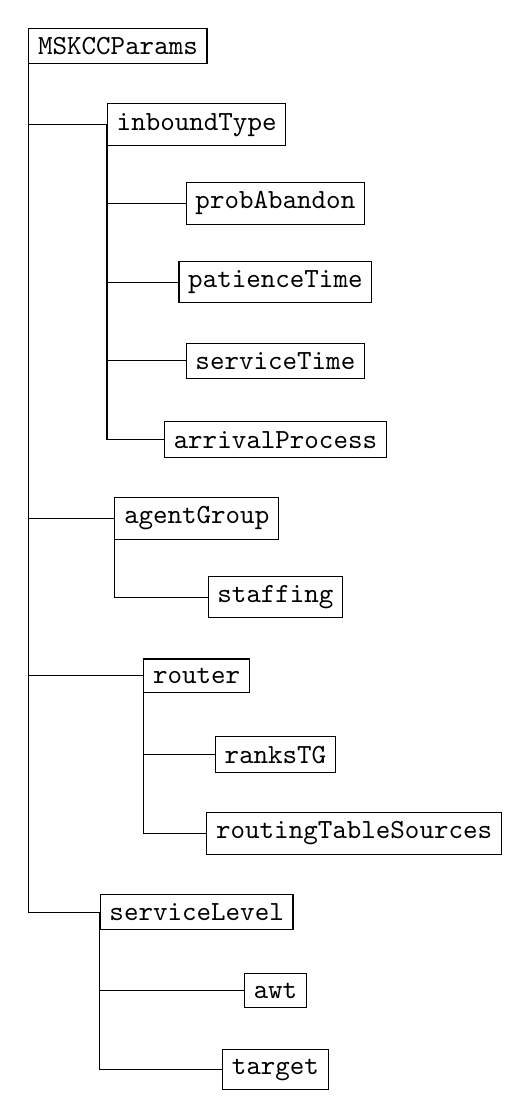
\begin{tikzpicture}[shape=rectangle,anchor=west]
\node (MSKCCParams) [draw] {\texttt{MSKCCParams}};
\node (inboundType) [draw, below of=MSKCCParams, xshift=1cm]
{\texttt{inboundType}};
\node (probAbandon) [draw, below of=inboundType, xshift=1cm]
{\texttt{probAbandon}};
\node (patienceTime) [draw, below of=probAbandon]
{\texttt{patienceTime}};
\node (serviceTime) [draw, below of=patienceTime]
{\texttt{serviceTime}};
\node (arrivalProcess) [draw, below of=serviceTime]
{\texttt{arrivalProcess}};
\node (agentGroup) [draw, below of=arrivalProcess, xshift=-1cm]
{\texttt{agentGroup}};
\node (staffing) [draw, below of=agentGroup, xshift=1cm]
{\texttt{staffing}};
\node (router) [draw, below of=staffing, xshift=-1cm]
{\texttt{router}};
\node (ranksTG) [draw, below of=router, xshift=1cm]
{\texttt{ranksTG}};
\node (routingTableSources) [draw, below of=ranksTG, xshift=1cm]
{\texttt{routingTableSources}};
\node (serviceLevel) [draw, below of=routingTableSources, xshift=-2cm]
{\texttt{serviceLevel}};
\node (awt) [draw, below of=serviceLevel, xshift=1cm]
{\texttt{awt}};
\node (target) [draw, below of=awt]
{\texttt{target}};

\draw (MSKCCParams.west) |- (inboundType)
(MSKCCParams.west) |- (agentGroup)
(MSKCCParams.west) |- (router)
(MSKCCParams.west) |- (serviceLevel);
\draw (inboundType.west) |- (probAbandon)
(inboundType.west) |- (patienceTime)
(inboundType.west) |- (serviceTime)
(inboundType.west) |- (arrivalProcess);
\draw (agentGroup.west) |- (staffing);
\draw (router.west) |- (ranksTG)
(router.west) |- (routingTableSources);
\draw (serviceLevel.west) |- (awt)
(serviceLevel.west) |- (target);
\end{tikzpicture}


\caption{The hierarchical structure of example in Listing~\ref{par:singleQueue}}
\label{fig:singleQueue}
\end{figure}

For call center parameters,
the name of the root element must be
\texttt{MSKCCParams}
%(see
%section~\ref{javadoc:umontreal.iro.lecuyer.contactcenters.msk.CallCenterParams})
with a namespace URI set to
\path{http://www.iro.umontreal.ca/lecuyer/contactcenters/msk}.
The \texttt{xmlns:ccmsk} attribute of this root element is used to
bind this URI to the shorter prefix \texttt{ccmsk} in the parameter
file.

The root element
is allowed to have some attributes such as
\texttt{period\-Duration} (main period duration
$d$),
%see p.~\pageref{javadoc:umontreal.iro.lecuyer.contactcenters.msk.CallCenterParams:getPeriodDuration()})
%and \texttt{queue\-Capacity} (maximal number of calls in queue) %, see
%p.~\pageref{javadoc:umontreal.iro.lecuyer.contactcenters.msk.CallCenterParams:getQueueCapacity()}),
\texttt{defaultUnit} (default time unit), etc.,
as well as children elements.
The attributes of an element are given after the name of the element,
and before the \texttt{>} marker.
Nested contents of the root element
is located between the
\lstinline[language=XML]!<ccmsk:MSKCCParams>!
and \lstinline[language=XML]!</ccmsk:MSKCCParams>! markers.

In this model, 13 periods of one hour are set up by setting
\texttt{num\-Periods} to 13 and \texttt{period\-Duration} to
\texttt{PT1H}.
The notation for time durations, which seems confusing at first
sight, is imposed by the XML Schema Specification (see
Section~\ref{sec:simpledatatypes}, and \cite[part 2, section
3.2.6]{iSPE00a}).
%The period
%duration must be set although it
%is unused for a stationary simulation, and conforms to the
%\texttt{duration} type defined by XML Schema .

The attribute
\texttt{default\-Unit},
%(see~p.~\pageref{javadoc:umontreal.iro.lecuyer.contactcenters.msk.CallCenterParams:getDefaultUnit()}),
set to \texttt{SECOND} in this example, sets the implicit unit
for time
durations.
This is the time unit used during simulation as well as the unit of
any time-related output, e.g., waiting time.

Nested elements are used to describe more complex information such
as call types, agent groups, the router, and the parameters
for estimating the service level.
The order of these elements must not be changed for the parameter file
to remain valid.
It is also important to keep the hierarchy of the document, e.g.,
the \texttt{router} element should not be moved inside an
\texttt{inbound\-Type} element.

We now describe the contents of the \texttt{inbound\-Type} element,
which represents the call type in this example, in more details.
First, the \texttt{name} attribute is used to bind a name to the
inbound call type.  A name can also be associated with an agent group.

The \texttt{prob\-Abandon} element is used to set the
probability of balking, for each main period.
This element accepts an array of values on the $[0,1]$ interval.
If the array contains a single value such as in this example, the
value is automatically reused for all
periods.  Therefore, the user does not need to repeat $0.1$ 13 times
to have $\rho=0.1$ for all periods in this example.

The way patience and service times are specified differ from the way
the period duration is given, because these aspects of the model
require probability
distributions, not only mean time durations.
The distribution for patience time is given using the
\texttt{patience\-Time} element
% (see
%p.~\pageref{javadoc:umontreal.iro.lecuyer.contactcenters.msk.CallTypeParams:getPatienceTime()})
whose type corresponds to a probability distribution.
% (see
%section~\ref{sec:probdist}).
  Such an element
accepts a
\texttt{distribution\-Class} attribute giving the SSJ class of the
probability distribution while the \texttt{default\-Gen} child element
sets the distribution parameters.
The latter element accepts an array giving
the arguments passed to the constructor of the chosen
distribution class.
The role of these arguments depends on the chosen distribution class,
and do not always correspond to means and variances.

Table~\ref{tab:maindist} gives the parameters for the
most commonly used distributions.
The first column gives the name of the class, i.e., the value of the
\texttt{distribution\-Class} attribute, corresponding to the
distribution.
The other columns give the density of the distribution, its
mean, its variance, and
the
order of parameters required for the
distribution.
See the package \path{umontreal.iro.lecuyer.probdist}
in the
user's manual of SSJ \cite{iLEC04j} for additional distributions.

\begin{table}
\caption{Parameters for the most commonly used probability distributions}
\label{tab:maindist}

\begin{center}
\begin{tabular}{|l|l|l|l|l|}\hline
\texttt{distributionClass} & Density $f(x)$ & Mean & Variance & Parameters \\ \hline
\texttt{ExponentialDist} & $\lambda e^{-\lambda x}$ for $x\ge
0$& $1/\lambda$ & $1/\lambda^2$ &
$\lambda>0$ \\
\texttt{ExponentialDistFromMean} & $e^{-x/\mu}/\mu$ for $x\ge
0$& $\mu$ & $\mu^2$ &
$\mu>0$ \\
\texttt{GammaDist} & $\lambda^{\alpha} x^{\alpha -
  1}\frac{e^{-\lambda x}}{\Gamma(\alpha)},$
for $x>0$ & $\alpha/\lambda$ & $\alpha/\lambda^2$ &
$\alpha>0$, $\lambda>0$ \\
\texttt{GammaDistFromMoments} &
 & $m$ & $v$ &
$m>0$, $v>0$ \\
\texttt{NormalDist} &
$\frac{\exp(-(x-\mu)^2/(2\sigma^2))}
         {\sqrt{2\pi}\sigma}$ &
$\mu$ & $\sigma^2$ &
$\mu$, $\sigma>0$ \\
\texttt{LognormalDist} &
  $\frac{\exp(-(\ln (x) - \mu)^2/(2\sigma^2))}{\sqrt{2\pi}\sigma x}$,
      &$e^{\mu+\sigma^2/2}$ & $e^{2\mu + \sigma^2}(e^{\sigma^2} - 1)$
& $\mu$, $\sigma>0$\\
&for   $x>0$
& && \\
\texttt{LognormalDistFromMoments}
& & $m$ & $v$ & $m>0$, $v>0$ \\
\hline
\end{tabular}
\end{center}

Here,
$    \Gamma (\alpha) = \int_0^\infty x^{\alpha-1} e^{-x} dx$.
In particular, $\Gamma(n) = (n-1)!$ when $n$ is a positive integer.

The gamma and lognormal distributions with moments have the same
density as the ordinary gamma and lognormal distributions, but a mean
and a variance are entered rather than shape and scale parameters.
\end{table}

According to Table~\ref{tab:maindist} or
the SSJ
documentation from \cite{iLEC04j}, the exponential
distribution is represented by the
\texttt{Exponential\-Dist\-From\-Mean} class,
and
has a scale parameter $\mu$ representing the mean
which needs to be
specified as an argument for calling the constructor.
%Since the \texttt{probdist} package was
%imported at the beginning of the XML file,
%the fully qualified class names of distributions do not need to be
%specified in \texttt{distribution\-Class} attributes.
Here,
$\mu=1000$.
The \texttt{unit} attribute of \texttt{patience\-Time} specifies that
the generated patience times must be considered in seconds, so
the mean patience time is 1000s for this example.
The \texttt{service\-Time} element % (see p.~\pageref{javadoc:umontreal.iro.lecuyer.contactcenters.msk.CallTypeParams:getServiceTime()})
has the same structure as
\texttt{patience\-Time}, but it gives the service time distribution for
calls, served by any agent.

The \texttt{arrival\-Process} element % (see Section~\ref{javadoc:umontreal.iro.lecuyer.contactcenters.msk.ArrivalProcessParams})
specifies the arrival process to
be used for this inbound call type, along with its parameters.
The \texttt{type} attribute is used to indicate the type of
arrival process, which can be any string specified in
Section~\ref{javadoc:umontreal.iro.lecuyer.contactcenters.app.ArrivalProcessType}.
The \texttt{arrivals} vector element gives the parameters for the
arrival process, in this case the Poisson arrival rate.
By default,
this arrival rate corresponds to the expected number of calls during a
simulation time unit, i.e., one second in our setting.
By setting the \texttt{normalize} attribute to \texttt{true}, we
instruct the simulator to interpret the arrival rates as relative to
one period.  Consequently, the given arrival rates set the expected
number of arrivals during each hour for this example.

The
\texttt{agent\-Group} element % (see Section~\ref{javadoc:umontreal.iro.lecuyer.contactcenters.msk.AgentGroupParams})
describes the agent group in the call
center.
The \texttt{staffing} child element is used to associate a staffing
with the agent group.
It contains an array giving the number of agents during each main
period of the day.
Alternatively, the array can contain a single element; the staffing
will then be fixed for the whole day.

Then, the \texttt{agent\-Group} element is used to describe the agent
group of the example.
We give a name to the agent group using the \texttt{name} attribute
and configure its staffing using the \texttt{staffing} element.
This gives a number of agents for each main period of the model.

The \texttt{router} element is then used to describe how routing is
done in the model.
Here, we have a very basic routing sending any incoming call to a free agent.
For this, the \texttt{router\-Policy} attribute is used to configure the
router's policy. Here, we use the \texttt{AGENTSPREF} policy which is
very general.
But we could use other more efficient policies for this example.
Section~\ref{javadoc:umontreal.iro.lecuyer.contactcenters.app.RouterPolicyType}
describes in details the
available router's policies.

The selected router's policy minimally requires a
$K\times I$ matrix associating a
priority to each (call type, agent group) pair during agent selection,
and
a second $I\times K$
matrix setting the priorities similarly during call
selection.
The first matrix is set using \texttt{ranksTG} (ranks for
type-to-group assignments)
while the second matrix is given using \texttt{ranksGT}
(ranks for group-to-type assignments).
A matrix can be represented by a sequence of arrays in the parameter
file, each array being represented by a \texttt{row} child element.
Here, we use the $1\times 1$ identity matrix for both parameters.
The second matrix can be given explicitly using the
\texttt{ranksGT}.
However, instead of transposing the contents of
\texttt{ranksTG} manually to obtain
\texttt{ranksGT} when $\rTG(k,i)=\rGT(i,k)$ for
all $k$ and $i$, we can instruct
the router to generate \texttt{ranksGT} by
transposing \texttt{ranksTG},
by using the \texttt{routing\-Table\-Sources} element.
This will become useful when we increase the number of call types and
agent groups.

The \texttt{service\-Level} element
%(see Section~\ref{javadoc:umontreal.iro.lecuyer.contactcenters.app.ServiceLevelParams})
gives thresholds for the service level using
two $\Ki'\times P'$
matrices: one for the acceptable waiting times, and a second one for the service
level targets.  Often, $\Ki'=\Ki+1$ if $\Ki>1$, and $\Ki$ otherwise,
and $P'$ is defined similarly using $P$.
Several \texttt{service\-Level} elements, with different
\texttt{awt} and \texttt{target} matrices, can
be specified to set the values for different contact types and
periods.
The targets are not considered during
simulation, but they can be used by
optimization programs.

However, these matrices are sometimes sparse, i.e., the user only
specifies some values.  Consequently, if a matrix of thresholds (or targets)
contains a single element, its single value is used for all call
types and periods.  If it contains a single row or column, the row or
column is duplicated as required.

Here, we set the acceptable waiting time to 20s, and the service level
target to 80\%.
We need $1\times 1$ matrix containing \texttt{PT20S}, and
\texttt{0.8}, respectively.
We also specify a second threshold of 30s with target 80\% by using a
second \texttt{service\-Level} element.

After the model parameters are configured, simulation parameters are
needed in order to perform experiments.
The simplest method of experiment consists of simulating a fixed
number of independent replications.  This can be described by a file
similar to
Listing~\ref{par:repSimParams}.

\lstinputlisting[caption={\texttt{repSimParams.xml}: Example of a
  parameter file for an
  experiment using independent replications}, language=XML%
,label=par:repSimParams]{repSimParams.xml}

The root element for the parameter file is \texttt{rep\-Sim\-Params} %(see
%Section~\ref{javadoc:umontreal.iro.lecuyer.contactcenters.app.RepSimParams}).
with namespace URI
\path{http://www.iro.umontreal.ca/lecuyer/contactcenters/app},
which differs from the namespace URI of \texttt{MSKCCParams}.
The number of performed runs is
fixed to 300 by the \texttt{min\-Replications}
attribute.

The \texttt{report} element % (see
%Section~\ref{javadoc:umontreal.iro.lecuyer.contactcenters.app.ReportParams})
contains the parameters of the statistical report produced by the
simulator.
In particular, the \texttt{confidence\-Level}
attribute sets the confidence
level of intervals to 95\%.
These confidence intervals are computed using the normal
assumption (see Section~\ref{sec:mskoutput}
for more details).
The report is printed when the simulator is invoked from the
command-line or when the \texttt{format\-Statistics} method is called
from a Java program.
This includes the confidence level of the printed intervals as well as
the statistics to include in the report.
Here, no information is provided about printed statistics so
the report includes information about all supported performance
measures.

\subsection{Variants of the single-queue model}

\subsubsection{Disabling abandonment}

In some situations, it can be necessary to disable abandonment, e.g.,
if no information about patience is available, or if simulation needs to
be compared with approximation formulas.
Doing this increases the workload of the simulated agents, because customers
abandoning must now all be served.
This increases the waiting time, and decreases the service level if
the number of agents is not increased to compensate for this.
Of course, a model without abandonment is less realistic than an
equivalent model with abandonment.

Abandonment can be disabled by
removing \texttt{prob\-Abandon} and \texttt{patience\-Time} from the
XML file.
Removing \texttt{prob\-Abandon} disables balking by setting the
probability of immediate abandonment to 0 while
removing \texttt{patience\-Time} sets all patience times to infinity.

Removing an element from a XML file can be performed by destructively
deleting all the text representing the element, and its children, or
by commenting it out. For example, the following code represents a
patience time which was commented out:
\begin{lstlisting}[language=XML]
<!--
      <patienceTime distributionClass="ExponentialDistFromMean" unit="SECOND">
         <defaultGen>1000</defaultGen>
      </patienceTime>
-->
\end{lstlisting}
The sequences \verb.<!--. and \verb.-->. serve as comment delimiters
in the XML language.  Since comments are ignored by the parameter
reader, they can be used to store additional information about the
parameter file.  This information is intended to be used by human
beings only.
Any information used by a computer program should be encoded in
XML elements, attributes, or nested text.

\subsubsection{Setting period-specific parameters}

The example on Listing~\ref{par:singleQueue} sets a stationary
distribution for the patience and service times.  If the distribution
of the service times can change from periods to periods, one can
replace the \texttt{default\-Gen} element of \texttt{service\-Time}
with a sequence of \texttt{period\-Gen} elements, as shown on the next
listing.
\begin{lstlisting}[language=XML]
      <serviceTime distributionClass="ExponentialDistFromMean"  unit="SECOND">
         <periodGen>100</periodGen>
         <periodGen>150</periodGen>
         <periodGen>180</periodGen>
         <periodGen>90</periodGen>
         <periodGen>110</periodGen>
      </serviceTime>
\end{lstlisting}
This sets the per-period mean service time, for a model defining five
main periods.
The $p$th \texttt{period\-Gen} element gives the parameters of the
service time for main period~$p$, with $p=1,\ldots,P$.
Of course, the number of \texttt{period\-Gen} elements must correspond
to the number of main periods in the model.

\subsubsection{Increasing the variability of arrivals}

\richard{Le d\'ebut de cette section doit \^etre r\'e\'ecrit pour tenir
compte de nos derni\`eres corrections: on peut inclure un facteur busyness
pour chaque type d'appel.}
With the arrival process of the original model, the number of arrivals
during period $p$ follows the Poisson distribution with mean
$\lambda_p$, and variance $\lambda_p$.
This variance can be increased randomizing the arrival rate in each
period.
The arrival process is then doubly stochastic.
For example, this can be done
by setting the arrival rates to
$B\lambda_p$, where $B$ is a random variable with mean 1.
The random variable $B$, generated each day,
represents the busyness factor of the day.
The day is more busy than usual when $B>1$ and less busy than usual
when $B<1$.
A well-studied distribution for $B$ is gamma with equal parameters
$\alpha_0$ \cite{ccAVR04a}.
Such a busyness factor can be used by adding the
\texttt{busyness\-Gen} element before any \texttt{inbound\-Type}
element, e.g.,
\begin{lstlisting}[language=XML]
   <busynessGen distributionClass="GammaDist">10 10</busynessGen>
\end{lstlisting}
This sets the distribution of the busyness factor to gamma(10,10).
This element does not accept \texttt{default\-Gen} or
\texttt{period\-Gen} children, because the busyness factor is
generated once at the beginning of the day, and thus does not change
from periods to periods.

Another way of increasing the variance of the number of arrivals is to
use a Poisson-gamma arrival process where the arrival rate for each
period is gamma-distributed, independently of other periods.
This can be specified as follows:
\begin{lstlisting}[language=XML]
      <arrivalProcess type="POISSONGAMMA" normalize="true">
         <poissonGammaShape>19 19 19 19 19 19 19 19
                            19 19 19 19 19</poissonGammaShape>
         <poissonGammaRate>100 150 150 180 200 150 150 150
                            120 100 80 70 60</poissonGammaRate>
      </arrivalProcess>
\end{lstlisting}
Here, we have changed the value of the \texttt{type} attribute to
\texttt{POISSONGAMMA}, and replaced the \texttt{arrivals} element
with \texttt{poisson\-Gamma\-Shape}, and
\texttt{poisson\-Gamma\-Rate}.
These new elements give the
gamma shape and rate parameters for each main
period.
Section~\ref{javadoc:umontreal.iro.lecuyer.contactcenters.app.ArrivalProcessType}
gives the list of all available arrival processes, with a detailed
description for each one.

\subsubsection{Changing the number of periods}

Increasing the number of periods often requires several updates in the
parameter file. First, the \texttt{num\-Periods} attribute in
\texttt{MSKCCParams} must be modified.
Then, each element defining period-specific parameters must be updated
with the new periods.
This includes balking probabilities
stored in \texttt{prob\-Abandon} elements,
patience and service times stored in
\texttt{patience\-Time} and \texttt{service\-Time} elements,
arrival process (\texttt{arrivals} elements for
Poisson processes with piecewise-constant rates), staffing
in \texttt{staffing} elements, and service
level information
in \texttt{service\-Level} elements.
Missing per-period parameters will result in error messages when
running the simulator.
If an element sets parameters for more periods than the value given by
\texttt{num\-Periods}, the last extra periods are ignored.
%TODO: print a warning in this case

\subsubsection{Adding a new call type}

Adding a new call type is a three-steps process:
\begin{enumerate}
\item Adding a new \texttt{inbound\-Type} element;
\item Adapting the routing policy for a new call type;
\item Extending the matrices of AWTs and targets for the service level.
\end{enumerate}
We now describe these steps in more details.

Adding a new \texttt{inbound\-Type} element can be done by copying the
contents of an existing \texttt{inbound\-Type} element, and
altering its contents.
The main issue to consider is the indexing of call types:
adding new call types can shift indices, and require adjustments in
other parts of the XML file.
More specifically, each call type receives an index based on its order
of occurrence in the XML file.
This index is used for specifying type-to-group and
group-to-type maps for some routing policies as well as
target call types for call transfers and virtual queueing.
See Section~\ref{sec:mskccParamsThreeTypes} for an example with a
type-to-group map.

In our original setting, the only call type has index 0.
Adding a new \texttt{inbound\-Type} element just below the original
one
creates a new call type with index 1.
However, adding the element \emph{before} the original
\texttt{inbound\-Type} element assigns index 0 to the new call type,
and shifts the index of the old call type to 1.
This can cause problems especially if the model already contains
several call types.

The second step in adding the call type is to update the parameters of
the routing policy.  In our example, we need to change
the
\texttt{ranksTG} child element of \texttt{router} in order to extend
the matrix of ranks with a new row.
This new row sets the priorities for the new
type.
Failing to do that will result in errors preventing the simulator to
run.

With a single agent group and
the agents' preference-based routing policy, if both call types have
the same priority,
agents becoming free select the call with the longest waiting time.
Otherwise, free agents first look for calls with the lowest rank
(i.e., highest priority) before calls with the highest rank.

If call type 1 has priority over call type 2, or even if
its mean service time is shorter than the mean service time of
call type 2,
calls of type~1 will wait less before they get service, and
therefore will have higher service level than
calls of type~2.

If both call types have the same priority, and mean service time, one
expects to get exactly the same results as with the model defining a
single call type.
In practice, results differ slightly because of the way random numbers
are generated by the simulator.
More specifically, sequences of random numbers are associated to each
call type separately.  By splitting the calls in two types,
one changes the number of constructed sequences of random streams, and
thus the generated random numbers.
Note that the difference between the single-type and the two-types model
decreases as the number of replications increases.

Extending matrices of AWTs and service level targets is optional if
it contains a single row, and the thresholds and targets do not depend
on the call type.
Otherwise, the matrices must contain one row per call type, plus a row
for the global parameters.

Listing~\ref{par:singleQueueTwoTypes} gives an example of a call
center with two call types, and one agent group.
Here, the target service level is 80\% for both types, but the AWT for
call type~2 is set to 60s.  The global AWT and target remain
at 20s, and 80\%, respectively.
In the new model, calls of type~1 have priority over calls of type~2.

\lstinputlisting[caption={\texttt{singleQueueTwoTypes.xml}: Example of
  a parameter file for a call center with a single agent group and two
call types}, language=XML%
,label=par:singleQueueTwoTypes]{singleQueueTwoTypes.xml}

\subsubsection{Adding a new agent group}
\label{sec:addAgentGroup}

Adding a new agent group involves two steps similar to adding a call
type:
\begin{enumerate}
\item Adding a new \texttt{agent\-Group} element;
\item Adapting the routing policy;
\end{enumerate}
We will now describe these steps in more details.

A new \texttt{agent\-Group} element can be added by copying an
existing element, and altering parameters.
Usually, the name and staffing of the agent group are adapted.
As with call types, adding agent groups can shift indices as we
discussed in the previous subsection.

The routing policy is adapted by adding a new column to
the matrix of ranks of the model.  This is done by updating the
\texttt{ranksTG} element in the parameter file.
This new column sets priorities concerning the new agent
group.
With a single call type, if two agent groups have the same priority,
a newly-arrived call is assigned to the agent with the longest idle
time among the two groups.
If ranks are different, the agent group with the lowest rank (i.e.,
highest priority) is checked for agents before the group with higher
rank.

Listing~\ref{par:singleQueueTwoGroups} gives an example of this
extension.  Here, we have added a second agent group, and set the
router for the first agent group to have priority over the second one.

\lstinputlisting[caption={\texttt{singleQueueTwoGroups.xml}: Example of
  a parameter file for a call center with two agent groups and a
single call type}, language=XML%
,label=par:singleQueueTwoGroups]{singleQueueTwoGroups.xml}

If we simulate with this parameter file, we obtain a warning about
agent groups not in detailed mode.  This is caused by the fact that in
general, the routing policy we have chosen requires the longest idle
times of agents to break tie for agent groups sharing the same minimal
rank.
This idle time can be obtained only when agent groups are in
detailed mode, i.e., if they model each agent as separate objects.
However, for this example, idle times are not needed, because all
ranks are different.

The warning can be removed two ways: by setting the
\texttt{detailed} attribute to \texttt{true}
for each \texttt{agent\-Group} element, or by
setting the \texttt{agent\-Selection\-Score} attribute of the
\texttt{router} element to something other than
\texttt{LONGESTIDLETIME}, e.g., \texttt{NUMFREEAGENTS}.
The first solution switches the agent groups to detailed mode, which
allows the idle times to be retrieved, while the second alternative
changes how tie is broken for agent groups sharing the same minimal
rank.

\subsubsection{Adding routing delays}

With the routing policy used in this model, agent groups are queried
sequentially in order to find a free agent to serve a newly-arrived
call; this is call \emph{overflow routing}.
Similarly, call types are looked up sequentially in order to find a
call for a free agent; this is denoted \emph{priority queueing}.
Sometimes, we need the router to wait for some time between each agent
group, and call type.  This can be done by setting delays in the
router's parameters.

First, the routing policy has to be switched from \texttt{AGENTSPREF}
to
\texttt{AGENTSPREFWITHDELAYS}.
Then, a $I\times K$ matrix of time durations is
specified using \texttt{delaysGT} element
Each element $(i, k)$ of the matrix gives the minimal time a call of
type~$k$ has to wait in queue before it can be served by any agent in
group~$i$.

As an example, suppose we combine the two extensions proposed in the
preceding subsections.  We therefore have two call types, and two
agent groups.
We then assign each call type $k=0,1$ a primary agent group $i$, but
we allow the other agent group to serve the call, with lower priority,
and a minimal delay of 30s.
The resulting \texttt{router} element looks as follows:
\begin{lstlisting}[language=XML]
   <router routerPolicy="AGENTSPREFWITHDELAYS">
     <ranksTG>
       <row>1   2</row>
       <row>2   1</row>
     </ranksTG>
     <delaysGT>
        <row> PT0S     PT30S</row>
        <row>PT30S      PT0S</row>
     </delaysGT>
     <routingTableSources ranksGT="ranksTG"/>
   </router>
\end{lstlisting}
Note that setting any rank for a $(k, i)$ pair
to $\infty$, by replacing the numerical
value with
\texttt{INF}, prevents the router from assigning
calls of type $k$ to agents in group $i$.

\subsubsection{Using agent schedules}
\label{sec:mskSchedules}

For any agent group described in a XML file representing call center
parameters, the staffing vector can be replaced with a schedule.
Schedules are composed of shifts to which
agents are assigned. The staffing vector is thus replaced with a vector
containing the number of agents per shift, with a description of the shifts.
The most common way of specifying schedule shifts is to give a
$J\times P$
matrix of booleans whose element $(j, p)$ is \texttt{true} if and only if
an agent working on shift $j$ is scheduled for main period~$p$.

Listing~\ref{par:singleQueueShifts} gives an example of an agent group
with a schedule. In this listing, the \texttt{staffing} element is
replaced with a \texttt{schedule} element containing a
\texttt{numAgents} child. This vector of agents instructs the simulator to
schedule one agent for each shift.
The matrix of shifts is set up using the element \texttt{shift\-Matrix}
which is placed after the element describing the agent group. Each row
of the matrix corresponds to a shift while each column concerns a main
period of the model.
The matrix of shifts is used for every agent group for which a schedule is
given.  Alternatively, one can give a matrix of shifts specific to an
agent group by putting a \texttt{shift\-Matrix} element inside the
\texttt{schedule} element, just before the \texttt{num\-Agents} element.

\lstinputlisting[caption={\texttt{singleQueueShifts.xml}: Example of
  a parameter file for a call center with a single agent group with
  a schedule, and a
single call type}, language=XML%
,label=par:singleQueueShifts]{singleQueueShifts.xml}

The simulator also accepts shifts represented as time
intervals. These are specified in the XML parameter file using
\texttt{shift} elements. For example, the first row of the
matrix of shifts in the above example may be written as follows.
\begin{lstlisting}[language=XML]
      <schedule>
         <shift numAgents="1">
            <shiftPart startingTime="PT8H" endingTime="PT12H" type="Working"/>
            <shiftPart startingTime="PT13H" endingTime="PT15H" type="Working"/>
         </shift>
      </schedule>
\end{lstlisting}
With this input method, the starting and ending times of shifts do not
need to match with a change of main period.

\subsubsection{Estimating parameters}
\label{sec:singleQueueMLE}

When modeling a call center, the probability
distributions of the random variables is unknown.
A common solution to this problem is to guess a parametric probability
distribution and fit real data to this distribution.
The generic simulator can estimate parameters from data for
probability distributions and some arrival processes by using
the maximum likelihood method.
For this, data can be specified directly in parameter files.
Listing~\ref{par:singleQueueMLE} presents the parameter file of the
example in Listing~\ref{par:singleQueue},
with some parameters replaced with artificial data.

\begin{lstlisting}[caption={\texttt{singleQueueMLE.xml}: Example of
  a parameter file with data for
  parameter estimation}, language=XML%
,label=par:singleQueueMLE]
<ccmsk:MSKCCParams defaultUnit="SECOND" periodDuration="PT1H"
                   numPeriods="13"      startingTime="PT8H"
     xmlns:ccmsk="http://www.iro.umontreal.ca/lecuyer/contactcenters/msk">
   <inboundType name="Inbound Type">
      <probAbandon>0.1</probAbandon>
      <patienceTime distributionClass="ExponentialDist" unit="SECOND">
         <defaultGen>0.001</defaultGen>
      </patienceTime>
      <serviceTime distributionClass="ExponentialDist" unit="SECOND">
     <!-- i.i.d. exponentials with lambda=0.01 -->
         <defaultGen estimateParameters="true">
   13.583  38.350  36.988  174.782  25.055  76.227  65.542  43.937
<!-- more observations here -->
</defaultGen>
      </serviceTime>
      <arrivalProcess type="PIECEWISECONSTANTPOISSON" normalize="true"
                      estimateBusyness="true">
        <!-- Observations generated from the Poisson distribution -->
         <data>
            <row>89 144 144 193 189 151 149 145 108 107 82 68 56</row>
            <row>93 153 166 173 175 173 137 158 110 86 73 74 53</row>
            <row>100 140 154 190 217 164 162 157 120 86 65 83 76</row>
            <row>99 153 155 143 222 146 151 157 125 89 81 58 66</row>
            <!-- More observations -->
         </data>
      </arrivalProcess>
   </inboundType>

   <agentGroup name="Inbound-only agents">
      <staffing>4 6 8 8 8 7 8 8 6 6 4 4 4</staffing>
   </agentGroup>

   <router routerPolicy="AGENTSPREF">
     <ranksTG>
       <row>1</row>
     </ranksTG>
     <routingTableSources ranksGT="ranksTG"/>
   </router>

   <serviceLevel>
      <awt>
         <row>PT20S</row>
      </awt>
      <target>
         <row>0.8</row>
      </target>
   </serviceLevel>
</ccmsk:MSKCCParams>
\end{lstlisting}

Data is specified at the same place as regular parameters, except that
the \texttt{estimate\-Parameters} attribute is set to \texttt{true}.
For probability
distributions over the real numbers (continuous or discrete), this
element is an array of double-precision values.
For discrete distributions over the integers, the double-precision
values of the data are rounded to the nearest integers.
%The \texttt{data} element can also be replaced by the \texttt{data\-URL}
%attribute which specifies the URL of a text file containing the data,
%one value per line.
%The URL can point to a local file, or a Web resource.
%Relative URLs are resolved using the location of the parameter file.
%Data can also be read from a CSV file or a database.
%See Section~\ref{sec:extarray} for more information.

For an arrival process, one must use the
\texttt{data} element which accepts a
matrix of integers giving the observed number of arrivals during each
main period for observed days.
The parameters of arrival processes are estimated by considering each
given
$P$-dimensional vector representing a day as independent and
identically distributed.

For arrival processes, parameter estimation is more complex, because
the number of arrivals in all periods comes from a multivariate
distribution, and some methods estimate the parameters of the busyness
factor and the arrival rates simultaneously.
For these reasons, the way parameters are estimated for arrival
processes depends on the specific type of process, and the value of
the \texttt{estimate\-Busyness} attribute.
For example, with the Poisson process with piecewise-constant arrival
rates, if the busyness factor is estimated, the number of arrivals is
assumed to follow the negative multinomial distribution, and a
gamma$(\alpha_0,\alpha_0)$ busyness factor is estimated.

Before the simulation starts, parameters are estimated using the
maximum likelihood method and used to create the
probability distributions; parameters are never displayed to the user.
If the results of the estimates need to
be known, a program is available to estimate parameters and produce a
new XML file representing the same model, with data replaced by
parameters.
See Section~\ref{sec:estparprg} for more information.

\subsection{Additional experiment parameters}

Listing~\ref{par:repSimParams} shows a very basic parameter file for
experiments with independent replications. By modifying
the \texttt{minReplications} and the \texttt{confidenceLevel}
attributes, we can change the number of replications to simulate and
the confidence level of intervals, respectively, but many other
parameters can be changed.  In this section, we give examples for the
most common changes.

\subsubsection{Getting a call-by-call trace}
\label{sec:trace}

Sometimes, it may be required to get a trace of every call processed
by the simulator.
This can be done by using the \texttt{call\-Trace} element in
experiment parameters as in Listing~\ref{par:repSimParamsTr}.
This parameter file indicates that 5 independent replications need to
be performed, and that a call-by-call trace has to be saved in the file
\texttt{test.log}.
The format of the trace file is plain text by default.
However, if one gives a file name ending with \texttt{.xls}, the trace
is stored into a spreadsheet compatible with Microsoft Excel.
Note that the \texttt{call\-Trace} element can also be used in
simulation parameters for batch means.

\lstinputlisting[caption={\texttt{repSimParamsTr.xml}: Example of a
  parameter file for an
  experiment using independent replications and producing a
  call-by-call trace}, language=XML%
,label=par:repSimParamsTr]{repSimParamsTr.xml}

%See
%Section~\ref{javadoc:umontreal.iro.lecuyer.contactcenters.app.CallTraceParams}
%for the exact contents of the trace.

\subsubsection{Restricting the printed statistics}

The \texttt{printed\-Stat} element % (see
%Section~\ref{javadoc:umontreal.iro.lecuyer.contactcenters.app.PrintedStatParams})
of \texttt{report}
indicates which performance measures
to print a report on.  During the simulation, statistics on all
supported performance measures are computed (see
Section~\ref{javadoc:umontreal.iro.lecuyer.contactcenters.app.PerformanceMeasureType}).
Listing~\ref{par:repSimParamsStat}
shows how to
indicate that we need a statistical report only for the
service level as well as the agents' occupancy ratio.  However, we do
not want a detailed report for the occupancy ratio: only the occupancy
ratio for all agent groups will be displayed.  But the
service level for each call type and period will be printed separately.
If no \texttt{printed\-Stat} element is given, a detailed report
for all supported performance measures is obtained.

\lstinputlisting[caption={\texttt{repSimParamsStat.xml}: Example of a
  parameter file for an
  experiment using independent replications and producing a report
  with selected statistics}, language=XML%
,label=par:repSimParamsStat]{repSimParamsStat.xml}

\subsubsection{Printing observations}

The simulator only computes statistics that do
not require the complete list of observations to be stored.
Consequently, observations are not stored in order to save memory.
However, in some situations, observations might be required, e.g.,
to estimate quantiles, plot histograms, etc.
The simulator therefore provides options to include observations for
selected performance measures into the generated report.
Measures have to be selected explicitly, because printing observations
for all measures would produce a huge report in which finding
the relevant information would be hard.

The list of observations are not available directly for performance measures
whose \texttt{EstimationType} is \texttt{FUNCTIONOFEXPECTATIONS}, as
for example \texttt{SERVICELEVEL}. For these, there is a closely related
performance measure with name suffix \texttt{REP},  of \texttt{EstimationType}
\texttt{EXPECTATIONOFFUNCTION}, for which the
complete list of observations may be collected by the simulator.
In the case of \texttt{SERVICELEVEL}, this measure is
\texttt{SERVICELEVELREP}.

Listing~\ref{par:repSimParamsObs} provides an example XML file for
printing observations.
First, the \texttt{keepObs} attribute has to be set to \texttt{true}
in order to instruct the simulator to keep observations.
Then, a \texttt{printedObs} element is added
for each performance measure for which observations are
desired.
The \texttt{row} and \texttt{column} attributes can be used to select
a specific row and column in the matrix of performance measures.
If they are omitted, observations are printed for the bottom-right
performance measure, which corresponds to the measure over all contact
types (or agent groups), and all time periods.

\lstinputlisting[caption={\texttt{repSimParamsObs.xml}: Example of a
  parameter file for an
  experiment using independent replications and producing a report
  with selected lists of observations}, language=XML%
,label=par:repSimParamsObs]{repSimParamsObs.xml}

Here, we select the number of served calls of any type,
the number of calls having abandoned,
and the number of calls of type 0 served after a waiting time
smaller than or equal to the acceptable waiting time.

\subsubsection{Changing random seeds}
\label{sec:seeds}

Although the simulation is stochastic, it always gives the same
results if it is performed with the same parameters.
This behavior is due to the fixed initial seed for random number
generators.
One can change this initial seed by using experiment parameters.
One can even use a different algorithm for generating uniform random
numbers.

For this,
the \texttt{random\-Streams} element is used to specify information
about random streams. In particular, the
optional \texttt{stream\-Seed} attribute allows one to set the
seed of random number generators for the simulation.  The value of
this attribute must correspond to an array given to the
\texttt{set\-Package\-Seed} static method of the selected random stream
class, \texttt{MRG32k3a} being the default.
These methods often take an array of integers as
argument.  With MRG32k3a, the default random number generator, one
needs an array of six integers to
represent the seed.
The optional attribute \texttt{stream\-Class} can be
used to specify a different class of random stream for generating
random numbers.  See the package \path{umontreal.iro.lecuyer.rng} in
the SSJ documentation \cite{iLEC04j} for more
information about available random streams.
Listing~\ref{par:repSimParamsSeed} gives an example of this.

\lstinputlisting[caption={\texttt{repSimParamsSeed.xml}: Example of a
  parameter file for an
  experiment using independent replications and different initial seed}, language=XML%
,label=par:repSimParamsSeed]{repSimParamsSeed.xml}

\subsubsection{Sequential sampling}

By default, the simulator performs a deterministic number of
replications set by the \texttt{min\-Replications} attribute, in
experiment parameters.
This becomes random if sequential sampling is used.
With this procedure, replications are performed until the target
relative error for selected performance measures falls below a
user-specified threshold.
More specifically, the simulator performs the minimal number of
replications, evaluates the relative error by dividing the half-width
of the confidence intervals by the point estimators, and estimates a
number of additional observations to generate.
This procedure continues until the relative error is smaller than the
targets for all selected performance measures, or a maximal number of
replications is reached.

Listing~\ref{par:repSimParamsSeqSamp} gives an example of a parameter
file for sequential sampling. Here, the element
\texttt{sequential\-Sampling} is used to select
performance measures for sequential sampling.
The \texttt{measure} attribute selects the service level as a group of measures.
For each main period of the model, we require that the relative error on
the service level be smaller than or equal to $1\%$, so the
attribute \texttt{target\-Error} is fixed to 0.01.
Confidence level on intervals used to estimate the relative errors are
computed with level given by the \texttt{confidence\-Level} attribute,
which can differ from the confidence level used for reporting.
Note that by setting the \texttt{global\-Only} attribute to
\texttt{true} in the \texttt{sequential\-Sampling} element, one could
select the overall service level only for sequential sampling rather
than the service level for all individual periods.

\lstinputlisting[caption={\texttt{repSimParamsSeqSamp.xml}: Example of a
  parameter file for an
  experiment using independent replications and sequential sampling}, language=XML%
,label=par:repSimParamsSeqSamp]{repSimParamsSeqSamp.xml}

\subsubsection{Parameters for the CTMC simulator}

The simplified CTMC simulator requires some additional parameters, for
example the length of the horizon used if simulating a single period.
Therefore, a parameter file similar to
Listing~\ref{par:repSimParamsCTMC} is needed.
A basic parameter file for the CTMC simulator is very similar to
regular files, except that an element with name
\texttt{ctmcrep\-Sim\-Params} rather than \texttt{rep\-Sim\-Params} is
used.
However, the \texttt{ctmcrep\-Sim\-Params} supports attributes and
child elements not supported by \texttt{rep\-Sim\-Params}.

\lstinputlisting[caption={\texttt{repSimParamsCTMC.xml}: Example of a
  parameter file for an
  experiment using independent replications and CTMC simulator}, language=XML%
,label=par:repSimParamsCTMC]{repSimParamsCTMC.xml}

In Listing~\ref{par:repSimParamsCTMC}, the attribute
\texttt{min\-Replications} instructs the simulator to perform 1000
replications while the attribute \texttt{time\-Horizon} sets the time
horizon to 13 hours. This time horizon is used by the single-period
CTMC simulator while the multi-period simulator uses the number of
periods and period duration to set the length of the horizon.

In addition to a special parameter file for experiment, the CTMC
simulator needs the queue capacity to be finite in the model.
This can be achieved by using the \texttt{queue\-Capacity} attribute
on the \texttt{MSKCCParams}. The XML file \texttt{single\-Queue\-CTMC}
shows an example of this.

\subsection{Stationary multi-skill call center}
\label{sec:mskccParamsThreeTypes}

This example, inspired from \cite{ccKOO00a} and presented on
Listing~\ref{par:mskccParamsThreeTypes},
represents a multi-skill call center
simulated for a single period.
The center has three call types and two agent
groups which can only serve two types of calls.
Every random variable is exponential and the routing
policy is static.

\lstinputlisting[caption={\texttt{mskccParamsThreeTypes.xml}: Example of
  a parameter file for a multi-skill stationary call center}, language=XML%
,label=par:mskccParamsThreeTypes]{mskccParamsThreeTypes.xml}

%The configuration file starts with the standard XML header specifying
%the version of XML to be used and the encoding.
%If this optional line is omitted, XML 1.0 is assumed, and the encoding
%of the file is considered to be UTF-8.
%This line is mandatory only when the XML file contains non-ASCII
%characters, e.g., accented characters in names of call types and agent
%groups.
%The following \texttt{import} lines correspond to \emph{processing
%  instructions} implemented by the parameter reader provided by the
%ContactCenters library.
%Some parameters in the XML file, e.g., probability distributions,
%accept a Java class name without assuming any implicit package name.
%As a result, without an import facility, the user would have to
%specify fully-qualified names every time, which would clutter its
%configuration files.  The \texttt{import} processing instruction
%provides this facility, allowing simple names to be
%inserted instead of fully qualified names.
%The imports work the same way as with the Java programming language.
%See the Java Language Specification \cite{iGOS00a} for more information.

Three \texttt{inbound\-Type} elements
% (see
%Section~\ref{javadoc:umontreal.iro.lecuyer.contactcenters.msk.InboundTypeParams})
follow the declaration
of the root element, each one describing an inbound call type~$k$.
%The \texttt{source\-Enabled} attribute (see p.~\pageref{javadoc:umontreal.iro.lecuyer.contactcenters.msk.CallTypeParams:getSourceEnabled()})
%indicates to the simulator
%that the arrival process producing calls of this type must be
%activated during a steady-state simulation.
These are similar to call type declarations in the preceding examples,
except we specified rates instead of means for patience and service
times.

For example, the patience rate for the first call type is set to 12,
which corresponds to a mean of $1/12$.
As set by the \texttt{unit} attribute, this mean must be interpreted
in hour, so the mean patience time is 5 minutes.

Here, we use the \texttt{QUEUEPRIORITY}
router's policy, for
which the \texttt{type\-To\-Group\-Map} and
\texttt{group\-To\-Type\-Map} elements are required.
The type-to-group map, in the \texttt{type\-To\-Group\-Map} element,
gives the order in which agent groups are
queried to serve each call type.  For example, a call of type~1 is served
by agents in groups~0 and~1.  If no agent in group~0 is free at the
arrival of the call, the
router checks for agents in group~1 before adding the call to a queue
corresponding to its type.
The group-to-type map, in the \texttt{group\-To\-Type\-Map} element,
determines in which queues to look for calls.
For example,
when an agent in group~0 becomes free, it looks for a call of type~1,
then for a call of type~0, and remains free if no call is available in
these queues.  This could also be achieved with the
\texttt{AGENTSPREF} policy, and the appropriate matrix of ranks, but the
\texttt{QUEUEPRIORITY} policy is faster.
However, the policy requires that each call type and agent group has a
different priority, which is more restrictive than the agents'
preference-based policy which allows shared priorities.
Note that this routing policy is not optimal;  it is
used for demonstration purposes only.

Here, we specify acceptable waiting times $\sK{k}$ for each call type
separately.  If the simulation was multi-period, the same AWT $\sK{k}$
would have been used for each period.  We also specify $s$, the
acceptable waiting time when estimating the service level for all call
types and periods.  Target service levels are specified the same way.

Here, we simulate a single long replication to estimate performance
measures as if the time horizon was infinite in the model, and we use
batch means to get estimates of variance and confidence intervals.
For this type of experiment, we need a parameter file similar to
the one presented in
Listing~\ref{par:batchSimParams}.
Simulation parameters determine the simulation length, warmup, and
reporting parameters.
In contrast, for previous examples, we used the parameter file
of Listing~\ref{par:repSimParams} for experiments, which gave the
number of independent replications to simulate.

\lstinputlisting[caption={\texttt{batchSimParams.xml}: Example of a
  parameter file for a stationary simulation}, language=XML%
,label=par:batchSimParams]{batchSimParams.xml}

The root element for batch means parameters is
\texttt{batch\-Sim\-Params} % (see
%Section~\ref{javadoc:umontreal.iro.lecuyer.contactcenters.app.BatchSimParams}).
with namespace URI \path{http://www.iro.umontreal.ca/lecuyer/contactcenters/app}.
%Since \texttt{target\-Error} (see
%p.~\pageref{javadoc:umontreal.iro.lecuyer.contactcenters.app.SimParams:getTargetError()})
%is negative in this
%example, error checking is disabled; the simulation length is
%fixed.
Simulation time is divided into batches of equal length \texttt{batch\-Size}
(20 hours in this example).  \texttt{warmup\-Batches} batches (5 in the
example) are simulated before statistical observations are collected in
order to reduce the bias of the estimators due to the transient period.
We hope that the system will have approximately reached steady-state after
this warmup is done.
To reach the steady-state more quickly, the system is initialized
non-empty:  the simulator tries to get 90\% of the agents busy before
the warmup period starts.
The total simulation time, in hours, is given by the formula
\texttt{batchSize*(minBatches + warmupBatches)}.

\subsection{Generalizing routing using matrices of ranks}
\label{sec:mskccParamsThreeTypesRanks}

As noted in the preceding example, the queue
priority router that we
used is more restricted but faster than the routing policy illustrated
in the first example.
In this section, we show how queue priority
routing can be obtained
using the agents' preference-based policy, and
give examples of what extensions can be made to this routing without
any Java programming.
For a detailed description of how this and other policies work,
see Section~\ref{javadoc:umontreal.iro.lecuyer.contactcenters.app.RouterPolicyType}.

First, we replace the \texttt{router} element in
Listing~\ref{par:mskccParamsThreeTypes} with the following one:
\begin{lstlisting}[language=XML]
   <router routerPolicy="AGENTSPREF">
     <ranksTG>
          <row>  2  INF</row>
          <row>  1    2</row>
          <row>INF  3</row>
     </ranksTG>
     <routingTableSources ranksGT="ranksTG"/>
   </router>
\end{lstlisting}

In contrast to the preceding example which uses queue priority,
the (equivalent) routing policy
of this example is configured to be agents' preference-based,
and a matrix of ranks is specified for agent selection only.
The other required matrix, used for contact selection, is then inferred
by transposing the given matrix because of the
instruction given by the \texttt{routing\-Table\-Sources} element.
In this example, row~$k$ of the matrix of ranks
gives information about
agent selection for new calls of type~$k$
whereas column~$i$ of the matrix affects
contact selection for any agent in group~$i$ becoming free.

In particular, for
new calls of type~0 and~2, only one agent group is tested for agents
since the matrix of ranks has a single column with a finite value on
rows~0 and~2.
For new calls of type~1, the first agent group has priority 1 while
the second group has priority 2.  Therefore, the first group is tested
for free agents before the second group.

Any agent of this model can serve two types of calls.
Consequently, each column of the matrix of ranks has only two rows
with a finite value.
For both columns, row~1 has the smallest value so both agent groups
give priority to calls of type~1.

Suppose that we change the above matrix by
setting $\rTG(0,0)=1$ and $\rTG(2,1)=2$.
This does not affect how calls select agent, but an agent becoming
free now has to select between two types of calls with the same
priority.
The default behavior in this situation is to select the call with the
longest waiting time.
One can also use the \texttt{weightsGT} element to give weights
$\wGT(i,k)$ to each waiting queue.
When an agent in group~$i$ becomes free, and call type~$k$ is tested,
the longest waiting time among calls of type~$k$ is multiplied by
$\wGT(i,k)$, and the router chooses the call with the longest weighted
waiting time.

We now return to the original matrix, and change
$\rTG(1,1)$ to 1.  Clearly, this has no impact on call selection, but
new calls of type~1 now have to choose between the two agent groups
with same priority.  The default behavior in this situation is to take
the agent with the longest idle time.
In a similar way to call selection, the \texttt{weightsTG} element may
be used to set weights $\wTG(k,i)$ multiplying idle times.

If all finite values of the matrix of ranks are set to 1, no
priorities are used for agent and call selection: new calls of type~1
select the agent with the longest idle time while free agents selects
the queued call with the longest idle time.

\subsection{Longest weighted waiting times}
\label{sec:sim2skill}

This example was inspired from the 2-Skill Simulator available from
\url{http://www.ccmath.com/Sim2Skill}.
The model contains two call types, and three agent groups.  Each call
type has its dedicated group of specialists for service, and a group
of generalists is available to serve both types when no specialist is
free.
The simulator available from the Web site uses Poisson arrival
processes as well as exponential patience and service times.  However,
the service rate depends on the call type and agent group, and the
routing policy can uses longest weighted waiting times.

For agent selection, the router uses overflow as in the preceding
examples, with an adapted type-to-group map.
However, contact selection uses a different routing policy called
\emph{longest weighted waiting time}.  With this policy,
when a specialist becomes free,
the router selects a contact of the appropriate type only.
However, a waiting queue must be selected in the case of generalists,
because the group-to-type map allows for generalists to select both
types of calls.  When both queues are non-empty, the router in this
example queries the first call in each queue, and
multiplies its waiting time by a \emph{queue weight}, also called a
\emph{waiting time factor}.  This weight is a constant depending on
the call type.  The router then selects the call with the
longest weighted waiting time.
By adjusting the weights properly, one can achieve a better balance of
service level between call types than when using queue priority
routing as in
the previous example.

Listing~\ref{par:sim2skill} gives the XML file for this example.  The
format of the file is similar to the format in the preceding example,
except there are two call types instead of three, and three agent
groups instead of two.  Agent groups have been given a name for
clearer statistical reports.

\lstinputlisting[caption={\texttt{sim2skill.xml}: Example of
  a parameter file for a call center with longest weighted waiting time router}, language=XML%
,label=par:sim2skill]{sim2skill.xml}

We have tried to match the results of our simulator with the results
obtained by using CCmath.  For this, we had to specify the same
parameters to both systems.  However, the format of the parameters
differs, because our model is more general than the CCmath's model.
Table~\ref{tab:sim2skillccmath} gives the parameters entered
in the Web form of CCmath with the corresponding XML elements in the
parameter file.

\begin{table}
\caption{Parameters in the Web form for CCmath with corresponding
  parameters in the \texttt{sim2skill.xml} file}
\label{tab:sim2skillccmath}
\begin{center}
\begin{tabular}{|l|rr|l|}\cline{2-3}
\multicolumn{1}{l}{}&\multicolumn{2}{|c|}{Skill}&\multicolumn{1}{l}{}\\
\cline{2-4}
\multicolumn{1}{l|}{}&1&2&XML element\\ \hline
Expected number of arrivals&6&2&\texttt{inboundType/arrivalProcess/arrivals}\\
Average service time specialists&1&0.8&\texttt{inboundType/serviceTime}\\
Average service time generalists&1.6&1.6&\texttt{inboundType/serviceTime}\\
Average time until abandonment&2&3.2&\texttt{inboundType/patienceTime}\\
Number of specialists&3&2&\texttt{agentGroup/staffing}\\
Waiting time factors&3&0.8&\texttt{router/queueWeights}\\
Acceptable waiting time&0.33&0.33&\texttt{serviceLevel}\\
Number of generalists&\multicolumn{2}{|r|}{4}&\texttt{agentGroup/staffing}\\
\hline
\end{tabular}
\end{center}
\end{table}

As with the preceding example, only a single period is set up, but
now, times are in minutes to match the times specified on the CCmath
Web form.  The period duration does not have a crucial importance,
because we simulate the model on an infinite horizon.
Most elements on the CCmath Web form can be mapped directly to XML
elements in the parameter file.
For example, the 2-minutes average patience
time for type 0 (skill 1 on the Web form) translates into a
\texttt{patienceTime} element
setting an exponential distribution with mean $2$.
Also note how the \texttt{group} attribute is used with
\texttt{service\-Time} elements to set the distribution of service
times for calls of a given type served by agents in specific groups.

The most important element present in the XML file but not on the Web form is
\texttt{router}.  We use the longest weighted waiting time routing policy
which asks for a type-to-group map, a group-to-type map, and weights
for each waiting queue.  The type-to-group map ensures that incoming
calls are routed to specialists first then overflow to generalists if
no specialist is available.  The group-to-type map ensures that free
specialists are assigned the appropriate call type, and free
generalists are assigned calls selected by the longest weighted
waiting time.
As we saw in the preceding section, we could also model this routing
using the more general agents' preference-based policy.

If we simulate the model both with CCmath and ContactCenters, we
obtain similar results.  Differences are caused by different random
seeds.
% Maybe a slightly different definition for service level?

If the weights are required to depend both on the call type and agent
group, one can use agents' preference-based routing instead of the
longest weighted waiting time policy used here.
Section~\ref{sec:mskInOutSim} presents an example using this policy,
although no weights are specified.

The CCmath simulator provides an additional routing option allowing
the reservation of agents:  one can specify that a certain number of
generalists are reserved for type-0 calls only.  Before a type-1 call
to be served by a generalist, the number of generalists must exceed
the number of reserved agents.  Our simulator does not provide an
equivalent routing policy, because there is no obvious way to
generalize it for more than two call types.
However, one could program a custom simulator with an adapted routing
policy for this.
%TODO: add example of this

\subsection{The local-specialist router's policy}
\label{sec:mskccParamsThreeTypesReg}

In this section, we extend the example in
Section~\ref{sec:mskccParamsThreeTypes} to
illustrate how to create a call center using the
local-specialist routing policy and is presented on
Listing~\ref{par:mskccParamsThreeTypesReg}.
To use the policy,
a region code is associated with each call type and agent group.  The
region of a call type corresponds to its \emph{originating region}
whereas the region of an agent group corresponds to its
\emph{location}.  The local-specialist routing policy tries to give
priority to routings in the same region while still allowing calls to
be served remotely.  For this example, we define a \emph{typeset} to be a
set of call types having the same name but possibly different
regions.  The same way, an agent \emph{groupset} is a set of agent groups
having the same name with possibly different regions.

When selecting an agent group for an incoming call, this policy gives
priority to agents in the same region as the caller.
If more than one local agent is available, it takes the one with the
smallest number of skills, i.e., the most specialist.
If there are several local agents with the same level of skill, the router
takes the agent with the longest idle time.

If the call cannot be served by a local agent, it is added to a
waiting queue corresponding to its type.  After a user-defined
overflow delay, the queued call becomes eligible for remote service if
it was not served locally.  As a result, a second agent selection
occurs, without requiring the serving agent to be in the same region
as the caller.

When an agent becomes free, it looks for a local queued call
he can serve.  If several calls are available, the one with the
longest waiting time is chosen.  If no queued call is available, the
agent checks for remote queued call having waited for a sufficiently
long time.  If no call is available, the agent remains free.

To use this policy, a region name must be associated with each call type
and agent group, by using custom properties.
Many elements of the model, in particular
call types and agent groups, can have a
\texttt{properties} child element which can specify any custom
property such as the region, the language, costs, etc.
Such a property contains a type, given by the name of the declaring element,
a name given by the \texttt{name} attribute, and has
an associated value
given by the \texttt{value} attribute, or nested text for
properties corresponding to arrays.
A local-specialist router can be specified using a type-to-group,
or using matrices of ranks.
We will use a matrix of ranks in this example since it is more general.

\lstinputlisting[caption={\texttt{mskccParamsThreeTypesReg.xml}: Example of
  a parameter file for a call center with local-specialist router}, language=XML%
,label=par:mskccParamsThreeTypesReg]{mskccParamsThreeTypesReg.xml}

This example is based on Listing~\ref{par:mskccParamsThreeTypes}, with
duplicated call types and
agent groups:  each original call type becomes a typeset
of two types,
while each
agent group becomes a groupset of two groups.
One set of call types and agent groups is located in
Montreal, while the second set is in Toronto.
In the \texttt{inbound\-Type} and \texttt{agent\-Group} elements, a
\texttt{properties} element is used to set a \texttt{region} string
which corresponds to the region name.
The first three call types originate from Montreal whereas the three
other types originate from Toronto.
The first two agent groups are located in Montreal whereas the others
are located in Toronto.
The call center has three call typesets and two agent groupsets.
The first typeset contains types~0 and~3, the second typeset contains
types~1 and~4, and the third typeset contains types~2 and~5.
The groupset~0 contains agent groups~0 and~2 whereas the second groupset
contains groups~1 and~3.
Note also the use of the \texttt{detailed} attribute to indicate that
the agent groups must be in detailed mode, which is is necessary to
get longest idle times.

The second information necessary to construct the router is the
skill count $s(i)$
of each agent group~$i$.  The \emph{skill count} corresponds
to the number of call typesets each agent group can serve.  In this
example, each agent group can serve two call typesets.
The last needed information is the overflow delay,
fixed to 6~seconds in this example,
and specifying the waiting time after which a call is allowed to be
served remotely.

With all this
information, a type-to-group map could be
constructed as shown in Listing~\ref{par:mskccParamsThreeTypesRegTG},
but we use a contact selection
matrices of ranks in this example.
This specifies a function $\rGT(i, k)$ giving the rank of agent group~$i$
for calls of type~$k$.  The lower the rank, the higher is the
preference or priority of the agents in the group~$i$ for call
type~$k$.
If $\rGT(i,k)=\infty$, agents in group~$i$ cannot serve calls of type~$k$.
This matrix, given by the \texttt{ranksGT} subelement of the
\texttt{router} element,
is used for contact selection while a second matrix,
defining a function $\rTG(k, i)$, is intended for agent selection.
In this example, $\rGT(i, k)=s(i)$ if agents in group~$i$ can serve
calls of type~$k$ and $\infty$ otherwise.

As with the first example, we need to tell the simulator to create the
type-to-group matrix of ranks by transposing the group-to-type
matrix of ranks, which is done by setting the \texttt{ranksTG} attribute to
\texttt{ranksGT} in the \texttt{routing\-Table\-Sources} element.

If we used a type-to-group map instead of a matrix of ranks,
we would create a type-to-group incidence matrix from the
type-to-group map.  This matrix indicates, for each $(k, i)$ pair, if
calls of type~$k$ can be served by agents in group~$i$.  Then, using
this incidence matrix and the skill counts, we create the
type-to-group matrix of ranks.
The group-to-type matrix of ranks is constructed by transposing the
type-to-group matrix of ranks.

\begin{lstlisting}[caption={Parameters for the local-specialist
    routing policy with type-to-group map equivalent to
    example in Listing~\ref{par:mskccParamsThreeTypesReg}},
  language=XML,
  label=par:mskccParamsThreeTypesRegTG]
   <router localSpecOverflowDelay="PT6S" routerPolicy="LOCALSPEC">
      <typeToGroupMap>
         <row>0  2</row>
         <row>0 1 2 3</row>
         <row>1 3</row>
         <row>2 0</row>
         <row>2 3 0 1</row>
         <row>3 1</row>
      </typeToGroupMap>
      <routingTableSources incidenceMatrixTG="typeToGroupMap"
                           ranksTG="incidenceMatrixTGAndSkillCounts"
                           ranksGT="ranksTG"/>
   </router>
\end{lstlisting}

According to the routing policy of this example,
calls of type~0 can be served by agents in group~0 and~2, calls of type~1 by
agents in all groups, etc.
Since for a fixed~$i$, the rank $\rGT(i, k)$ is equal for all~$k$ where
$\rGT(i, k)<\infty$, as soon as an agent
becomes free, it takes the call with the longest waiting time it can
serve.

Several interesting extensions to this example can be imagined.
For example, agents in groupset~0 may be more generalists than agents
in groupset~1.  This can be modeled by increasing the skill count of
agent groups~1 and~3.
if $s(1)$ and $s(3)$ become 6, when a call of typeset~1
arrives, the router selects agent groupset~0 instead of~1 if there
are agents in the former groupset.  In the original setting, if there are
agents in both groupsets, the agent with the longest idle time is chosen.

Agents in groupset~0 may be better at serving calls of typeset~0 than
calls of typeset~1, independently of the region.  This could be
indicated in the matrix of ranks by setting $\rGT(0, 0)=\rGT(0, 3)=\rGT(2,
0)=\rGT(2,3)=1$, and letting the other values of the original matrix
unchanged.  For groupset~0,
we decrease the rank for typeset~0 to 1 while keeping the rank at 2
for the other typeset.  This modification
would not change the agent selection, but instead of taking the call with
the longest waiting time when an agent in the first groupset (groups~0
and~2) becomes free, the router would give priority to calls of the
first typeset (types~0 and~3) and take the longest waiting time for the
other call typesets.

In addition, changing the local-specialist routing policy to
agents' preference-based policy removes the local aspect
of the routing.
The \texttt{AGENTSPREF} routing policy can model completely static
schemes such as overflow push routing with queue priority pull routing
as in the previous example, completely dynamic schemes
assigning incoming calls to the longest idle agents and pulling the
queued calls with the longest waiting time, or a mixture of these
extremes.

The \texttt{AGENTSPREFWITHDELAYS} routing policy is a further
generalization of this permitting the service of a call by an agent
only after the call has spent a minimal delay in queue.
Listing~\ref{par:mskccParamsThreeTypesRegDelays} shows a
\texttt{router} element specifying agents' preference-based routing with
a delays matrix equivalent to
the local-specialist routing policy.
The key idea is to set the delay to 0 for local call-to-agent
associations, and 6s
for remote associations.

\begin{lstlisting}[caption={Parameters for the agents'
    preference-based routing policy with delays equivalent to
    local-specialist}, language=XML,
  label=par:mskccParamsThreeTypesRegDelays]
   <router routerPolicy="AGENTSPREFWITHDELAYS">
      <ranksGT>
         <row>  2     2 INF   2     2 INF</row>
         <row>INF     2   2 INF     2   2</row>
         <row>  2     2 INF   2     2 INF</row>
         <row>INF     2   2 INF     2   2</row>
      </ranksGT>
      <delaysGT>
         <row>PT0S PT0S PT0S PT6S PT6S PT6S</row>
         <row>PT0S PT0S PT0S PT6S PT6S PT6S</row>
         <row>PT6S PT6S PT6S PT0S PT0S PT0S</row>
         <row>PT6S PT6S PT6S PT0S PT0S PT0S</row>
      </delaysGT>
      <routingTableSources ranksTG="ranksGT"/>
   </router>
\end{lstlisting}

\subsection{More complex routing policies}
\label{sec:mskComplexRouting}

In the preceding sections, we have presented examples using routing
policies based on simple parameters, namely matrices of priorities,
and lists of contact types and agent groups.
These policies cover a large number of cases, but some situations
require more complex routing.
In particular, the preference of an agent group for a new call
might depend on some conditions on the system while the priorities of
queued calls might change during its waiting time.
In general, such complex
routing requires programming a custom policy. We present a simple
example of this in Section~\ref{sec:mskCustomRouting}.
However, for some cases, a predefined policy named
\texttt{OVERFLOWANDPRIORITY} might be enough.

% For each new call, this policy executes a kind of script determining
% the preference of agent groups for the new call, and the queue it
% waits in if not served immediately, at different predetermined times
% while the call is waiting in queue.

This policy works by computing two vectors of
ranks for each new call as well as for each
call queued for a sufficiently
long time.
The pairs of vectors of ranks are computed at fixed
waiting times, also called rerouting
times.
There is one
vector of ranks for agent selection, and an
optional vector of ranks for queue priority.
If the second vector of ranks is omitted, it defaults to the first vector.
The vector for agent selection determines the preference of the call for each agent group,
while the vector for queueing
fixes the priority of the call in each queue if it cannot be served at the time the
vectors are computed.
In general, the vectors can depend on conditions on the state of the call
center, but we first consider cases where the vectors are fixed.

After vectors of ranks are obtained,
the router selects the agent group with the smallest finite rank (which
corresponds to the highest preference), but containing at least one
free agent.  An infinite rank for an agent group $i$ means that the
call cannot be served by agents in group~$i$ at the current stage of
routing.
If an agent group can be found for the call, the call is removed from
any queue it is waiting in, and sent to an agent.
Otherwise,
the call is queued at every agent group for which the rank is finite.
The call stays in queue until it gets served, abandons, or its waiting
time reaches the threshold for the next routing stage.

With this routing policy, there is one waiting queue per agent group,
plus an extra queue for calls not authorized to be served during some
periods of time (we will come on that later).  The calls in queues
linked to agent groups are sorted in descending order of priority, i.e.,
ascending value of rank. This means that high-priority calls go before
low-priority ones.
Calls sharing the same priority are sorted in
increasing order of time spent in queue.
Therefore, an agent becoming free simply takes the first call in the
queue.
Note that the call can wait in several queues simultaneously, can move
from queues to queues during its waiting time, or its priority in some
queues can change with time.

We now present some examples using this policy.
We start with an example using a single queue, and no condition, to
show how priorities can change with waiting time.
We then continue with an example with two queues, and show how to
implement conditional routing.
For a more detailed description of how the policy works, see
Section~\ref{javadoc:umontreal.iro.lecuyer.contactcenters.app.RouterPolicyType}.
See also the complex type \texttt{Call\-Type\-Routing\-Params}, in the
HTML documentation of the XML Schema for the complete syntax
of routing parameters, including how to encode conditions.

\subsubsection{A single waiting queue, two call types}

Suppose for this example that calls are partitioned into two
types. The first type represents regulated calls, for which we need to
obtain a proportion of 80\% of calls served within a
waiting time limit of 20
seconds.
For the second type of calls, we do not have this constraint on the
service level, but we would like a small average waiting time.
In the model, all agents can serve all calls.

A first idea of routing policy for such a situation is to ensure that
agents serve regulated calls with higher priority than non-regulated
ones. We can easily obtain this by using the \texttt{AGENTSPREF} policy, with
a $1\times 2$ matrix of ranks assigning a priority of 1 to regulated
calls, and a priority of 2 to other calls.
We recall that the lower is the rank, the higher is the priority.
We can achieve the same routing using the \texttt{OVERFLOWANDPRIORITY}
policy, with the appropriate routing scripts for the two call types.

Listing~\ref{par:op-singleQueue} presents a parameter file
implementing this model, with parameters for both policies.
In practice, the \texttt{OVERFLOWANDPRIORITY} policy should not be
used if another simpler policy allows one to perform the exact same
routing, because the more complex policy we present in this subsection
is also slower to run.
Moreover, we will see that the syntax of routing scripts is more
verbose than the one for parameters of simpler policies.
We present this example for demonstration purposes, and as a basis for
more complex examples.

\lstinputlisting[caption={\texttt{op-singleQueue.xml}: Example of
  a configuration file using the \texttt{OVERFLOW\-AND\-PRIORITY} routing
  policy
  giving priority to a call type over the other one}, language=XML%
,label=par:op-singleQueue]{op-singleQueue.xml}

The parameter file first indicates that the horizon is divided in 22
periods of half an hour.
It then describes the two call types of the
example in a way similar to preceding files.
These call types share the same parameters, except the
arrival process. Although the call types have exactly the same arrival
rates in their respective \texttt{arrivals} elements, they have a
different arrival rate multiplier, given by their
\texttt{arrivals\-Mult} attributes. This multiplier gives a factor by
which each arrival rate is multiplied.
For this example, the multiplier of arrival rates of the regulated
calls is 25\% while the other multiplier is 75\%.
This means that 25\% of the total volume of calls corresponds
to regulated calls while the other 75\% is non-regulated calls.

After the two call types, the parameter file describes the agent group
and assigns it a staffing vector.
This is exactly the same as in previous parameter files.

The description of the routing comes after this.
The parameter file gives two descriptions of the exact same routing,
one with the simpler \texttt{AGENTSPREF} policy, one with the more
complex \texttt{OVERFLOWANDPRIORITY} policy.
The first description is commented, and included only for
demonstration purposes; it is not needed for the parameter file to be
valid.
First note the difference in complexity of the two policies. While
\texttt{AGENTSPREF} only requires a $1\times 2$ matrix, the
\texttt{OVERFLOWANDPRIORITY} policy needs a full script for each call
type.

The parameters of this router correspond, for each call type, to a
script composed of stages.  The simplest way to describe a stage is
by a waiting time at which vectors of ranks are computed,
a mandatory vector of ranks for agent selection, and
an optional vector for queue priority.
Each call-type specific script is represented, in the XML parameter
file, by an element with name \texttt{call\-Type\-Routing}.
Stages are represented by \texttt{stage} elements with a
\texttt{waiting\-Time} attribute giving the waiting time of the stage.
The \texttt{stage} element also includes
a \texttt{default} child containing an element with name
\texttt{agent\-Group\-Ranks} giving the mandatory vector of ranks.
The optional vector, not used here, would be given by
adding a child named \texttt{queue\-Ranks} to the \texttt{default}
element.

For our example, each call type has a single-stage script assigning
a fixed rank
at waiting time 0, i.e., at arrival time.  Regulated
calls receive a rank of 1 to have high priority while non-regulated
calls get a rank of 2. This does not affect how calls are sent to
agents in the single group, but this affects the order of calls in the
queue.

\subsubsection{Priorities changing with waiting time}

Suppose now that the priority of calls evolve with the waiting time
according to the following rules:
\begin{itemize}
\item The priority of any new call entering the queue is 3.
\item The priority of any regulated call waiting more than 10 seconds
  becomes 2.
\item The priority of any non-regulated call waiting more than 20 seconds becomes
  2.
\item The priority of any call waiting more than 100 seconds is
  changed to 1.
\end{itemize}

This scheme can be implemented using either
\texttt{AGENTSPREFWITHDELAYS} or \texttt{OVERFLOW\-AND\-PRIORITY}
policies.
Listing~\ref{par:op-singleQueue-cp} shows the required parameters for
both policies. The other parameters of the model are the same as in
Listing~\ref{par:op-singleQueue}.

\begin{lstlisting}[caption={Part of \texttt{op-singleQueue-cp.xml}:
    routing parameters for an example of priorities of calls evolving with waiting
  time}, label=par:op-singleQueue-cp, language=XML]
<!--  <router routerPolicy="AGENTSPREFWITHDELAYS">
    <ranksGT>
      <row>3  3</row>
    </ranksGT>
    <ranksGTUpdate minWaitingTime="PT10S">
      <row>2  3</row>
    </ranksGTUpdate>
    <ranksGTUpdate minWaitingTime="PT20S">
      <row>2 2</row>
    </ranksGTUpdate>
    <ranksGTUpdate minWaitingTime="PT100S">
      <row>1  1</row>
    </ranksGTUpdate>
    <routingTableSources ranksTG="ranksGT" ranksGT="ranksTG"/>
  </router> -->
  <router routerPolicy="OVERFLOWANDPRIORITY">
    <!-- Routing script for regulated calls -->
    <callTypeRouting>
      <stage waitingTime="PT0S">
        <default>
          <agentGroupRanks>3</agentGroupRanks>
        </default>
      </stage>
      <stage waitingTime="PT10S">
        <default>
          <agentGroupRanks>2</agentGroupRanks>
        </default>
      </stage>
      <stage waitingTime="PT100S">
        <default>
          <agentGroupRanks>1</agentGroupRanks>
        </default>
      </stage>
    </callTypeRouting>
    <!-- Routing script for non-regulated calls -->
    <callTypeRouting>
      <stage waitingTime="PT0S">
        <default>
          <agentGroupRanks>3</agentGroupRanks>
        </default>
      </stage>
      <stage waitingTime="PT20S">
        <default>
          <agentGroupRanks>2</agentGroupRanks>
        </default>
      </stage>
      <stage waitingTime="PT100S">
        <default>
          <agentGroupRanks>1</agentGroupRanks>
        </default>
      </stage>
    </callTypeRouting>
  </router>
\end{lstlisting}

In addition to delays, the \texttt{AGENTSPREFWITHDELAYS} policy
accepts alternate matrices of ranks used when the waiting time of a
call reaches a given threshold.
To implement the above routing, we need the four following different
matrices of ranks:
\begin{itemize}
\item The usual matrix, encoded with the \texttt{ranksGT} element, and
  used to set a rank of 3 for any newly queued call.
\item The first alternate matrix, encoded with the
  \texttt{ranksGTUpdate} element with a \texttt{min\-Waiting\-Time}
  attribute corresponding to 10 seconds, which sets the priority of
  regulated calls waiting more than 10 seconds to 2, and keeps the old
  priority of 3 for non-regulated calls.
\item The second alternate matrix, which sets the priority of
  non-regulated calls to 2 at 20 seconds of wait, and keeps the old
  priority of 2 for non-regulated calls.
\item The last alternate matrix
  setting the priority of all calls queued for more than 100
  seconds to 1.
\end{itemize}
For a more detailed description of how the routing policy works with
multiple matrices of ranks, see its documentation in
Section~\ref{javadoc:umontreal.iro.lecuyer.contactcenters.app.RouterPolicyType}.

To perform the same routing using
\texttt{OVERFLOWANDPRIORITY},
we need multiple stages for both call types.
Each stage, encoded in the parameter file using a
\texttt{stage} element, corresponds to a change of priority, with a threshold on
the waiting time set by the \texttt{waiting\-Time} attribute, and
a new priority given by the one-element vector
\texttt{agent\-Group\-Ranks}.

\subsubsection{Two call types and agent groups}

Our next example has two call types, and two agent groups.
Suppose that 10\% of the total volume of calls have type \texttt{Small}, and
the other calls have type \texttt{Large}.
There is a group of primary agents for each of the two call types, but
a call waiting more than 30 seconds can be served by any agent.
However, agents give priority to their primary call type.
Listing~\ref{par:op-twoQueues} gives an example of parameter file for
this model.

\lstinputlisting[caption={\texttt{op-twoQueues.xml}: Example of
  a configuration file using the \texttt{OVERFLOW\-AND\-PRIORITY} routing
  policy, with two call types and agent groups}, language=XML%
,label=par:op-twoQueues]{op-twoQueues.xml}

The beginning of the file is similar to
Listing~\ref{par:op-singleQueue}, except that we describe two agent
groups instead of a single one, and the names of call types and agent
groups are different.

Then, the routing parameters for the \texttt{AGENTSPREFWITHDELAYS}
and \texttt{OVERFLOWANDPRIORITY} policies are given.
For the first policy,
we first need a $2\times 2$ matrix of ranks with 1's on the diagonal
and 2 on the two other elements. This matrix indicates that
calls can
be served by any agent, but, for $k=1,2$, new calls of type~$k$ prefer agents
in group~$k$, and free agents in group~$k$ pick up queued calls of
type~$k$ with higher priority than calls of the other type.
A complementary $2\times 2$ matrix of delays is used to indicate that overflow
only occur for calls waiting more than 30 seconds.
The matrix of delays thus has 0 on its diagonal, and 30 on the other
elements.

To get the same routing with \texttt{OVERFLOWANDPRIORITYROUTER},
we need a different script for the two call types.
For call type 1, the first stage, at waiting time 0, indicates that
the vector of ranks is $(1, \infty)$.  This means that a new call of
the first type has access to agents in the first group but not in the
second group. If the call cannot be served immediately, it is queued
at first group with priority 1.
If it waits more than 30 seconds before getting served or abandoning,
the second stage of the routing occurs.
In this case, the vector of ranks is $(1, 2)$, which means that the
call still has access to the first agent group, but it can also be
served by an agent in the second group.
If the call still cannot be served, it is kept in the queue at the
first agent group, but it is also queued at priority 2 at the second
agent group.
A similar routing script is used for the second call type, with
different vectors of ranks.

Note that we could have changed the priority in \emph{both} queues at a given
stage. For example, if the vector of ranks was $(2,2)$ rather than
$(1,2)$, this would mean that the priority of the call in the queue
corresponding to its primary agent group would decrease rather than
staying fixed.

We now present more complicated examples that cannot be obtained using
other predefined policies than \texttt{OVERFLOWANDPRIORITY}.

\subsubsection{Simulating routing and transfer delays}

First, we suppose that the routing of a new call as well as overflow
take 5 seconds each, and that after a call overflows from the
primary agent group to the secondary group, it cannot be served
anymore by a primary agent.  In such a case, we say that the call is
\emph{transferred} from its primary to its secondary queue.

More specifically, a call arriving in the system must wait 5
seconds before it is queued at its primary agent group.
Then, if the call does not get service in the next 30 seconds, it is
transferred to the secondary queue. But during the 5-seconds
transfer process, the call cannot be served by any agent.
The call can abandon at any time during the process, even during the
routing and transfer times.

Listing~\ref{par:op-twoQueues-slowOv} gives the XML code necessary to
implement the above routing.
The other parameters of the model are the same as
in Listing~\ref{par:op-twoQueues}.
As with previous examples in this subsection, we can obtain the
appropriate routing by describing a list of stages for each call type,
each stage being defined by a threshold on the waiting time, and a
vector of ranks.

\begin{lstlisting}[caption={Part of \texttt{op-twoQueues-slowOv.xml}:
    parameters of a routing policy including routing delays and
    transfer times},
language=XML, label=par:op-twoQueues-slowOv]
  <router routerPolicy="OVERFLOWANDPRIORITY">
    <!-- Routing script for first call type -->
    <callTypeRouting>
      <stage waitingTime="PT5S">
        <default>
          <agentGroupRanks>1   INF</agentGroupRanks>
        </default>
      </stage>
      <stage waitingTime="PT35S">
        <default>
          <agentGroupRanks>INF  INF</agentGroupRanks>
        </default>
      </stage>
      <stage waitingTime="PT40S">
        <default>
          <agentGroupRanks>INF  2</agentGroupRanks>
        </default>
      </stage>
    </callTypeRouting>
    <!-- Routing script for second call type -->
    <callTypeRouting>
      <stage waitingTime="PT5S">
        <default>
          <agentGroupRanks>INF   1</agentGroupRanks>
        </default>
      </stage>
      <stage waitingTime="PT35S">
        <default>
          <agentGroupRanks>INF  INF</agentGroupRanks>
        </default>
      </stage>
      <stage waitingTime="PT40S">
        <default>
          <agentGroupRanks>2  INF</agentGroupRanks>
        </default>
      </stage>
    </callTypeRouting>
  </router>
\end{lstlisting}

One may notice in this listing that for some stages, the vector of
ranks is $(\infty, \infty)$, which means that the call has access to
no agent until the next stage. This also implies that the call is not
in any queue linked to an agent group.
In such cases, the router keeps a trace of the call in an extra queue
no agent group has access to.  As soon as the waiting time is large
enough to reach the next stage of routing, the call leaves this extra
queue, and joins back a queue linked to an agent group.
Of course, the call can also abandon while in the extra queue.

\subsubsection{Conditional routing}

We finish this subsection with two examples of conditional routing in
which the vectors of ranks for some stages are not fixed.
In general,
for each call type and each threshold on the waiting time, the
parameters of the routing define a list of cases, each case being
composed of a
condition, along with the two vectors of ranks.
The condition can depend on the size of waiting queues, the fraction of
busy agents in groups, and even statistics observed during a given
time window preceding the decision.
The router checks each condition in the order given by the cases, and
takes the vectors of ranks corresponding to the first true condition.
In addition to these cases, one can give a default set of vectors
which is used when no condition applies, or if no condition is given.
If no condition applies, and no default set of vectors is given, nothing
happens at the corresponding stage of routing; the call stays in queue
until the next stage, service, or abandonment.

Because of conditional routing, the description of a routing stage can
be more complex than what we saw so far.
In addition to the threshold on the waiting time represented by the
\texttt{waiting\-Time} attribute, a \texttt{stage} element
includes
a list of \texttt{case} children with conditions, a mandatory vector
of ranks for agent selection, and an optional vector for queue priority.
Moreover, one can omit the
default case with vectors of ranks but no condition,
and represented by the \texttt{default} element we saw in
previous examples.
Conditions are also expressed using XML elements and attributes; we
now show examples of this.

We now return to example in Listing~\ref{par:op-twoQueues}.
Suppose that when a call has spent 30 seconds in queue, it gains
access to the secondary agent group if and only if
the size of the queue associated with this secondary group is smaller
than 5, and less than 25\% of the agents available in the secondary
group are busy.

To implement this, we need to replace the \texttt{default} element in
the second stage of every routing script by a \texttt{case} element
giving appropriate conditions in addition to the vector of ranks.
Listing~\ref{par:op-twoQueues-cond} shows the routing parameters for this.

\begin{lstlisting}[caption={Part of \texttt{op-twoQueues-cond.xml}:
    example of parameters for conditional routing},
language=XML, label=par:op-twoQueues-cond]
  <router routerPolicy="OVERFLOWANDPRIORITY">
    <!-- Routing script for first call type -->
    <callTypeRouting>
      <stage waitingTime="PT0S">
        <default>
          <agentGroupRanks>1   INF</agentGroupRanks>
        </default>
      </stage>
      <stage waitingTime="PT30S">
        <case>
          <all>
            <queueSizeThresh index="1" threshold="5" rel="SMALLER"/>
            <fracBusyAgentsThresh index="1" threshold="0.25" rel="SMALLER"/>
          </all>
          <agentGroupRanks>1   2</agentGroupRanks>
        </case>
      </stage>
    </callTypeRouting>
    <!-- Routing script for second call type -->
    <callTypeRouting>
      <stage waitingTime="PT0S">
        <default>
          <agentGroupRanks>INF   1</agentGroupRanks>
        </default>
      </stage>
      <stage waitingTime="PT30S">
        <case>
          <all>
            <queueSizeThresh index="0" threshold="5" rel="SMALLER"/>
            <fracBusyAgentsThresh index="0" threshold="0.25" rel="SMALLER"/>
          </all>
          <agentGroupRanks>2   1</agentGroupRanks>
        </case>
      </stage>
    </callTypeRouting>
  </router>
\end{lstlisting}

For both call types, we use the \texttt{all} condition which accepts
a list of conditions being tested at decision times.  The \texttt{all}
condition is true only if all the nested conditions are true.
This is equivalent to an ``and'' condition.
Each \texttt{all} condition of the example contains two elements:
\texttt{queue\-Size\-Thresh} used to describe a
condition on the queue size, and
\texttt{frac\-Busy\-Agents\-Thresh} used for a condition on the
fraction of busy agents.
For each of these two conditions, we need to give the index of the
checked waiting queue or agent group, the threshold value, and the
relationship to check.
Other similar conditions can be given, e.g., for checking that the size
of the first waiting queue is greater than the size of the second one.

For another example of conditional routing, suppose that
a call of type $k$ whose waiting time reaches 30 seconds gains access to the
secondary agent group if and only if service level of calls of type
$k$ with acceptable waiting time of 20 seconds, observed during the
last 5 minutes, is smaller than 60\%.
This routing can be obtained by replacing the conditions in the
parameters
of Listing~\ref{par:op-twoQueues-cond}.
The new parameters are shown in
Listing~\ref{par:op-twoQueues-condStat}.

\begin{lstlisting}[caption={Part of
    \texttt{op-twoQueues-condStat.xml}: example of parameters for
    conditional routing depending on the service level observed during
  the last 5 minutes}, language=XML, label=par:op-twoQueues-condStat]
  <router routerPolicy="OVERFLOWANDPRIORITY">
    <!-- Routing script for first call type -->
    <callTypeRouting>
      <stage waitingTime="PT0S">
        <default>
          <agentGroupRanks>1   INF</agentGroupRanks>
        </default>
      </stage>
      <stage waitingTime="PT30S">
        <case>
          <stat measure="SERVICELEVEL" numCheckedPeriods="5"
                checkedPeriodDuration="PT1M">
               <statWithThresh index="0" threshold="0.6" rel="SMALLER"/>
            </stat>
          <agentGroupRanks>1   2</agentGroupRanks>
        </case>
      </stage>
    </callTypeRouting>
    <!-- Routing script for second call type -->
    <callTypeRouting>
      <stage waitingTime="PT0S">
        <default>
          <agentGroupRanks>INF   1</agentGroupRanks>
        </default>
      </stage>
      <stage waitingTime="PT30S">
        <case>
          <stat measure="SERVICELEVEL" numCheckedPeriods="5"
                checkedPeriodDuration="PT1M">
               <statWithThresh index="1" threshold="0.6" rel="SMALLER"/>
            </stat>
          <agentGroupRanks>2   1</agentGroupRanks>
        </case>
      </stage>
    </callTypeRouting>
  </router>
\end{lstlisting}

In this listing,
the \texttt{all} condition is replaced by the \texttt{stat} condition,
which requires the name of a type of performance measure
(\texttt{SERVICELEVEL} in this example), the number of checked
periods (5 here), and the duration of checked periods (1 minute in
this example). The contents of the \texttt{stat}
 element describes which performance
measures of the given type are checked.
Here, we indicate by using a \texttt{stat\-With\-Thresh} element
that we need the service level to be smaller than a
threshold.
The call type to which we check the service level is identified by the
\texttt{index} attribute while the threshold is set up using the
\texttt{threshold} attribute.

Note that the statistics for conditions are collected the same way as
global statistics which appear in reports produced by the simulator.
As a consequence, the acceptable waiting time for the service level is
taken from the same \texttt{service\-Level} element as the default
output of the simulator.

Other conditions can be used for routing.
For example, we could check that the service level for the first call
type is greater than the one for the second call type.
Conditions can also be applied on other statistics such as the average
waiting time, the abandonment ratio, etc.
Moreover, the \texttt{either} and \texttt{all} elements can be used
and nested to construct complex conditions checking several state
variables of the system.
For a description of the syntax used to encode conditions,
see the complex type \texttt{Routing\-Case\-Params} in the
HTML documentation of the XML Schemas of ContactCenters.

\begin{comment}
\subsection{Non-stationary single-skill call center}
\label{sec:mskCC}

This example comes from the SSJ User's Guide \cite{iLEC04j} and models
a call center with a single call type, a single agent group, but
multiple periods.  It is also presented in another guide of this
library, with a complete Java program using ContactCenters directly
rather than the generic simulator.
Each day, the center operates for $P$ hours.  The arrival rate of
calls and the number of agents answering them vary during the day, but
they are constant within each hour.

Calls arrive following a Poisson process with piecewise-constant
randomized arrival rate $B\lambda_p$ during period~$p$, where
$\lambda_p$ is
constant and $B$ is a random variable having the gamma distribution with
parameters $(\alpha_0, \alpha_0)$.
Thus, $B$ has mean~1 and
variance~$1/\alpha_0$, and it represents the busyness of the day.
The day is more busy than usual when $B>1$ and less busy than usual
when $B<1$.
This arrival process is studied in \cite{ccAVR04a}.

Calls that cannot be served immediately are put in a FIFO queue as in
the previous example, and callers can abandon.  The i.i.d.\ patience
times are generated as follows: with probability $\rho$, the patience
time is 0, i.e., the caller abandons if he cannot be served
immediately.  With probability $1-\rho$, the patience time is
exponential with mean $1/\nu$.  Service times are i.i.d.\ gamma random
variables with shape parameter~$\alpha$, scale parameter~$\gamma$,
and mean~$\alpha/\gamma$.

During main period~$p$, $N_p$ agents are available to serve calls.
If, at the end of period~$p$, the number of busy agents is
larger than $N_{p+1}$, ongoing calls are completed, but new
calls are not accepted until the number of busy agents is smaller than
$N_{p+1}$.  During the preliminary period, there is no agent whereas
for the wrap-up period, $N_{P+1}=N_P$.
Listing~\ref{par:mskCC} presents the XML file for this example.

\lstinputlisting[caption={\texttt{mskCC.xml}: Example of
  a parameter file for a non-stationary single-skill call center}, language=XML%
,label=par:mskCC]{mskCC.xml}

The most important difference from preceding examples is the multiple
periods configured by setting \texttt{num\-Periods} to 13, and the
\texttt{period\-Duration} to one hour.
Each simulation time unit corresponds, in this example, to one second
because of the \texttt{default\-Unit} parameter.

For the busyness $B$, we have to specify a generator
through the element \texttt{busyness\-Gen}.  The parameter file instructs
the simulator to generate $B$ following a gamma distribution with
equal parameters.
The arrival rates are specified in the \texttt{arrivals} element of
the arrival process.

The probability of balking must be set to $\rho$ for each period.
When the \texttt{prob\-Abandon} array contains a single element, it
is repeated implicitly as many times as required.
This convenience avoids one to repeat the same value of $\rho$ 13
times.
This also happens with other arrays such as \texttt{staffing}.
Other parameters are specified the same way as in preceding examples.

The simulator could of course use batch means parameters with this
model.  In this case, it would use the parameters of the first period
and estimate
steady-state performance measures.  The \texttt{current\-Period}
attribute in
\texttt{batch\-Sim\-Params} %(see
%p.~\pageref{javadoc:umontreal.iro.lecuyer.contactcenters.app.BatchSimParams:getCurrentPeriod()})
allows the simulated period to be specified, rather than using the
default which is 0.
One could simulate in steady-state for every period separately to get
estimates for every period, but this does not consider the correlation
between periods.
In this case, it is better to simulate independent replications to get results
for a finite horizon.

\subsection{Non-stationary multi-skill call center}
\label{sec:mskSimple}

This example, taken from \cite{ccBUI05a} and presented on
Listing~\ref{par:mskSimple}, models a simple
multi-skill but non-stationary call center.
We consider a center with three contact types, two
agent groups, and three two-hour periods.  Contacts
of type~$k$ arrive
following a Poisson process with randomized piecewise-constant arrival
rates
$B\lambda_{k, p}$ during
period~$p$, where the $\lambda_{k, p}$ are constants,
and $B$ is a gamma random variable with parameters
$(\alpha_0,\alpha_0)$ as in the preceding example.

When a contact arrives, an agent is selected from a group depending on
its type.  Contacts of type~0 can only be served by agents in
group~0 while contacts of type~2 can only be served by agents in
group~1.  Contacts of type~1 are served by agents in group~0, or
agents in group~1 if no agents are free in group~0.
Service times are i.i.d.\ exponential variables
with mean~$1/\mu_p$ for contacts arriving during period~$p$.
Agents in each group~$i$ are not differentiated, and
$N_{i,p}$ changes between periods while being constant within each period.

A contact that cannot be served immediately is added to a waiting
queue corresponding to its type.  Abandonment is supported, with
patience times that are i.i.d.\ exponentials with mean~$1/\nu_p$
for contacts arriving during period~$p$.

\lstinputlisting[caption={\texttt{mskSimple.xml}: Example of
  a parameter file for a non-stationary multi-skill call center}, language=XML%
,label=par:mskSimple]{mskSimple.xml}

As in the preceding examples, this XML file specifies several periods.
Each simulation time unit corresponds, in this example, to one minute
because of the \texttt{default\-Unit} parameter.
The busyness generator is set the same way as in the preceding
example, even though
the same value of $B$ is used for the three arrival
processes.

The three call types only differ by their arrival rates in this
parameter file.  The probability of balking is set to 0 for the three
periods so the \texttt{prob\-Abandon} elements are omitted.

% The \texttt{service\-Time} element contains no information, except
% from a single attribute.
% An element having the \texttt{xref} attribute cannot have any
% other attribute or nested contents.  In the parameter file, a
% compatible element
% having an \texttt{id} attribute whose value is the same as the value
% of \texttt{xref} must be set.  In this exemple, below the three
% call types, \texttt{rvg} elements with the correct \texttt{id} are
% declared.  This is used to postpone the definition of service time
% distribution and have each call type use the same parameters without
% repeating them.  Note that the service times are still independent
% random variates, even though the information about the distribution is
% shared.

% Parameters such as probabilities of balking, arrival rates, patience
% rates, service rates, and staffing vectors
% are given for the three mains periods.

The \texttt{router} uses the single FIFO queue policy with appropriate
routing tables.  This is similar to queue priority, except that the
call with the longest waiting time is selected when an agent becomes
free rather than pulling the call from the first queue.
As a result, the order of call types in the
group-to-type map can be freely changed, since it has no importance
for this particular routing policy.

Finally, we give a global acceptable waiting time and a service
level target, using the \texttt{service\-Level} element at the bottom
of the file.
\end{comment}

\subsection{Blend call center model}
\label{sec:mskBlend}

This example, adapted from \cite{ccDES07a} and presented on
Listing~\ref{par:mskBlendSim}, represents a blend call
center with two call types and two agent groups.
The simulated day starts at 8AM, ends at 2PM, and is
divided into three two-hours periods.
This call center supports outbound calls in addition to inbound ones.
Outbound calls are produced by using a predictive
dialer taking into account the state of the system to determine at any
time how many calls to try.
A first group of agents is capable of serving inbound calls only while
a second group of blend agents can serve both types of calls.

\lstinputlisting[caption={\texttt{mskBlendSim.xml}: Example of
  a parameter file for a blend call center}, language=XML%
,label=par:mskBlendSim]{mskBlendSim.xml}

We set \texttt{num\-Periods} to 3 and the
\texttt{period\-Duration} to two hours.
The \texttt{prob\-Abandon} element in the \texttt{inbound\-Type} element
fixes the probability of balking to $0.005$ for each period.

We took most input values from Table~2 in \cite{ccDES07a}, at
periods~15, 16, and~17.
For the three periods, the exponential patience time is set to 500
seconds.  For the parameter file, we have to
use the exponential distribution accepting a mean, and specify
\texttt{SECOND} as the time unit.

For the service times of inbound calls, we use a gamma distribution.
According to Table~\ref{tab:maindist}, this distribution,
implemented by the \texttt{Gamma\-Dist} class, has a
shape parameter $\alpha$, a scale parameter $\lambda$, and mean
$\alpha/\lambda$.  In the
paper from which the input values were taken, the used gamma has the
same shape
parameter but the scale parameter is $\beta=1/\gamma$.  To feed the
input to the SSJ's gamma distribution, we therefore need to invert the
scale parameters in the input data.
The order of the two parameters,
namely $\alpha$ followed by
$\lambda$,
depends on the \texttt{Gamma\-Dist}
constructor which is specified in SSJ's documentation.

By default, SSJ uses inversion to generate gamma variates, which
is rather slow.  To speed up generation, we use the
\texttt{generator\-Class} attribute to switch to
acceptance-rejection.  The appropriate class is described in the
\path{umontreal.iro.lecuyer.randvar} package of SSJ.
As with the patience time, the time unit is set to one second for
service times to be in seconds.

The \texttt{source\-Toggle\-Time} element
% (see
%p.~\pageref{javadoc:umontreal.iro.lecuyer.contactcenters.msk.CallTypeParams:getSourceToggleTimes()})
specifies an interval, in simulation time units, during which
the arrival process is enabled, i.e., produces calls.
Note that an arrival process can have an unbounded number
of \texttt{source\-Toggle\-Time} elements defining non-overlapping
intervals.
This mechanism therefore provides a way to extend
the model to a multiple-days horizon.
If no source toggle times are given, the arrival process
is enabled during all the main periods of the horizon.
In this example,
arrivals start 5 minutes before the call center opens for a waiting
queue to build up before 8AM, and
stops at 2PM, which corresponds to the time the call center
closes.

The number of agents is 0 in both groups until the preliminary period
ends and the call center opens.
For other random variates,
parameters are taken from the first main period if values are needed
before 8AM.
At 8AM, the first main period, which corresponds to the first period
where parameters are available, starts.

The arrival process is configured to be Poisson
with piecewise-constant arrival rates specified in
the \texttt{arrivals} vector.
% (see
%p.~\pageref{javadoc:umontreal.iro.lecuyer.contactcenters.app.ArrivalProcessType:PIECEWISECONSTANTPOISSON}).
From the input data, we have the average number of arrivals per half hour.
The \texttt{arrivals} element needs the arrival rate according to the
default time unit, i.e., hours in this example.  We therefore multiply
the input arrival rates by 2 to get hourly rates.

For outbound calls, the probability of balking is set
to 1, and patience time is omitted.
As a result, a mismatched call is dropped without
waiting in queue.
We need the mean service time of outbound calls to be 440.2~seconds.
If we assume exponential service times, the appropriate rate
is obtained by inverting the mean and the time unit is set to
\texttt{SECOND}.
We decided to start the dialer at 11AM and to stop it 5 minutes
before the center closes.

The rest of the outbound type parameters describes the dialer being
used, with a \texttt{dialer} subelement.
% (see
%Section~\ref{javadoc:umontreal.iro.lecuyer.contactcenters.msk.DialerParams}).
The \texttt{DIALXFREE} threshold-based dialer policy (see
p.~\pageref{javadoc:umontreal.iro.lecuyer.contactcenters.app.DialerPolicyType:DIALXFREE})
is applied to
determine the number of calls to dial.
This policy computes the total number of free agents $\Ntf(t)$ in all groups
(inbound and blend), and checks that this number is
greater than or equal to the minimal number of free agents (4 in this
example) given by the
\texttt{min\-Free\-Agents\-Test} attribute.
% (see
%p.~\pageref{javadoc:umontreal.iro.lecuyer.contactcenters.msk.DialerParams:getMinFreeAgentsTest()}).
It also verifies that the number of free blend agents $\Ndf[1](t)$
is greater than or equal to a second threshold set by the attribute
\texttt{min\-Free\-Agents\-Target}.
% (see
%p.~\pageref{javadoc:umontreal.iro.lecuyer.contactcenters.msk.DialerParams:getMinFreeAgentsTarget()}).
In this example, because the attribute is unspecified, the default value of 1 is used.
If these conditions hold,
the policy multiples $\Ndf[1](t)$ by $\kappa$, a multiplicative
constant
set by the \texttt{kappa} attribute which
equals~2 in this example.
It rounds $\kappa\Ndf[1](t)$ to the nearest integer and adds $c=0$ to it.
If this number is positive, this gives the number of calls to dial.
Otherwise, no call is dialed.
The dialer starts each time a service ends during the time internal it
is enabled.
See
Section~\ref{javadoc:umontreal.iro.lecuyer.contactcenters.app.DialerPolicyType}
for more information about available dialer's policies.

The \texttt{prob\-Reach} element
%(see
%p.~\pageref{javadoc:umontreal.iro.lecuyer.contactcenters.msk.DialerParams:getProbReach()})
specifies the probabilities of successful contact, for each period.
By default, the dial delay of calls is set to 0, whether the call is successful or
not.  One can use the \texttt{reach\-Time} and \texttt{fail\-Time}
% (see
%p.~\pageref{javadoc:umontreal.iro.lecuyer.contactcenters.msk.DialerParams:getFailTime()})
elements to provide non-zero dial delays.

The inbound-only and blend agent groups are then specified, with their
respective staffing vectors.  Each staffing vector contains three
values representing the number of agents for each period.

Here, the routing scheme is completely static:
if an inbound call arrives, it is served by an inbound-only agent or a
blend one if no inbound-only agent is available.
Outbound calls are served by blend agents only.
When an inbound-only agent becomes free, it looks for an inbound call.
Free blend agents look for outbound calls first, then for inbound ones.

\subsection{Blend and multi-skill call center}
\label{sec:mskInOutSim}

This example, presented on Listing~\ref{par:mskInOutSim},
demonstrates most of the aspects of the model implemented
by the simulator.
It does not correspond to a real call center model;
its only purpose is to demonstrate the capabilities of the simulator.
The call center is opened from 9AM to 2PM and its opening time is
divided into five one-hour periods.
Two inbound and two outbound call types, along with four agent groups,
are specified.  Agents in the first group are trained for inbound calls
only whereas agents in the second group are outbound-only.  The two
remaining agent groups contain blend agents skilled for serving one
type of inbound calls and one type of outbound ones.
Blend agents are less efficient than inbound-only or outbound-only,
because they are considered less specialized.
The routing policy must be configured to accommodate this preference, and
a longer service time occurs when the less specialized blend agents are
used.

More specifically,
inbound calls of type~$k$, for $k=0,1$, are served by inbound
agents in group~0, or blend agents in group~$k+2$ if no inbound agents
are available.
In a similar way, outbound calls of type~$k$, for $k=2,3$, are served
by outbound agents in group~1, or blend agents in group~$k$
if no outbound agent is available.
An inbound [respectively outbound] agent becoming free serves the
inbound [outbound] call with the longest waiting time.
Blend agents always give priority to outbound calls over inbound
calls.

\lstinputlisting[caption={\texttt{mskInOutSim.xml}: Example of
  a parameter file for
  a blend and multi-skill call center}, language=XML%
,label=par:mskInOutSim]{mskInOutSim.xml}

The first inbound call type uses a Poisson arrival
process with a period-specific arrival rate.  As in the
preceding example, there is no busyness generator.
The first inbound call type can be served by inbound-only agents
(group~0) as well as the first group of blend agents (group~3).
To reward services by specialists, the service rate with inbound-only
agents (group~0) is higher than with blend agents.
The probability of balking changes during each period, and
the exponential abandonment rate is set to 12 as in the first example
so mean patience time is 5 minutes.
Calls of this type arrive during all the opening hours of the call
center because of the \texttt{source\-Toggle\-Time} element.

The second inbound call type shows other aspects of the model.
First, the activity of the arrival process occurs during two
non-overlapping time intervals: from 9AM to 10h12AM and
from 10h48AM to 2PM.
%Note that the times are in decimal, not in hours, minutes, and seconds,
%in the parameter file.  These are time durations relative to the
%beginning of the horizon rather than absolute times.  As a result,
%$0.2$ hours is mapped to $12$ minutes.
Again, there is a probability of immediate abandonment for each period
and a service rate for each agent group.
Note that the service time distribution could, as with the preceding
example, be different for each period, even if we are using the
\texttt{group} attribute.  However, the \texttt{group} attribute
is allowed in the \texttt{service\-Time} element only, not in
the \texttt{period\-Gen} subelements.
Calls of this type arrive following a Poisson-gamma arrival process.
%(see
%p.~\pageref{javadoc:umontreal.iro.lecuyer.contactcenters.app.ArrivalProcessType:POISSONGAMMA}).
When this process is used, at the beginning of each day,
for period~$p$, the arrival rate is generated following a gamma distribution
with shape parameter $\alpha_{\mathrm{G}, p}$ and scale parameter
$\lambda_{\mathrm{G}, p}$ (mean~$\alpha_{\mathrm{G},
  p}/\lambda_{\mathrm{G}, p}$).
The shape parameters are given using
\texttt{poisson\-Gamma\-Shape} while the rate parameters
are set using \texttt{poisson\-Gamma\-Rate}.

The first outbound call type (also denoted call type~2 in the call type
index space) is then set up.
As with the preceding call types, a service time
distribution for each agent group is specified.
The dialer producing calls of this type starts at 12AM and stops at
2PM, and, as in the previous example,
the \texttt{DIALXFREE} threshold-based dialer's policy
is applied to
determine the number of calls to dial.
We fix the threshold for free agents in the test set to 4,
and keep the default of 1 for the free agents in the target set.
The multiplicative constant is set
to $\kappa=2$, and the additive constant, to $c=0$.
We recall that $\Ndf[2](t)$ is the number of
free agents in the outbound-only group (group~1),
and the first blend group (group~2).

The second call type is described in the same way as the first one, with
different parameters.
The dialer starts at 11h30AM and stops at 1h30PM.
Although it would be possible to use a different dialing policy,
we use the policy as with the preceding call type, with
different parameters.
The minimal number of free agents (in all agent groups) required to
allow dialing is
fixed to 3 whereas the multiplicative constant is $\kappa=2.5$, and additive
constant is $c=1$.
The target group from which the number of free agents $\Ndf[3](t)$ is
obtained is composed of the outbound-only group (group~1) and the
second blend group (group~3).

The parameter file then describes the four agent groups with a different
staffing vector for each one.
Each agent group also has a name for clearer statistical reporting.
We already showed a few examples of routing using matrices of ranks.
See for example Section~\ref{sec:mskccParamsThreeTypesRanks}.
Therefore, we will not detail here how the matrices of ranks are
used.

\begin{comment}
The staffing vector of the first agent group is computed from a
schedule instead of being specified explicitly.
This schedule, set by the \texttt{schedule} element and applied to
all members of the group. gives a set of \emph{shifts}
encoded in the parameter file as \texttt{shift} elements.
Each shift is described as a set of time intervals also called
parts, and encoded as \texttt{shiftPart} elements, and
specifies the number of working agents.
Each part has an associated starting and ending times as well as
a type name.
The type indicates what agents
do during the interval.
At this time, \texttt{Working} is the only part type used by the
simulator.  Any other part type results in agents not being staffed
during the concerned period.

% When specifying time intervals, one only gives the starting period,
% because the ending period is automatically inferred from the start
% period of the next part.  This has two important consequences: shift
% parts must be ordered by ascending value of the starting period, and
% the last part is used to get the (non-inclusive) ending period of the
% shift only.
% Note also that all period indices specify main periods.

For example, the first shift specified in the schedule of the example
starts at 9AM.  A break starts at
11AM (i.e., beginning of
period~2), so agents work during periods~0, and 1.
The break ends at the beginning of period~3, and the agents work for
two additional periods at the end of this shift.
If this was the only specified shift, the resulting staffing vector
would be $(1, 1, 0, 1, 1)$.

The combination of the described shifts results in the staffing vector
specified in
the XML file. This is only a sample schedule; many other (maybe more
efficient) schedules would result in the same staffing vector.
% Note that if one uncomments the \texttt{staffing} element and
% specifies a
% different staffing vector, this staffing vector would take precedence
% over the implicit vector computed from the schedule.
\end{comment}

\begin{comment}
The routing policy is configured to be agents' preference-based,
and a matrix of ranks is specified for contact selection only.
The other required matrix is then inferred by transposing the given
matrix.
When an inbound call arrives, inbound-only agents have priority
over blend agents to serve the call since they are more efficient at
this task.  As a result, in column~0 of the matrix of ranks, representing priorities
for call type~0 (first inbound type), element at row~0, representing
the inbound-only agent group,
has a lower rank than element at row~2, which represents the first blend agent group.
Column~1 (for call type~1, i.e.,
second inbound type) is similar to column~0, except that agent group~3
is used instead of agent group~2.
When an outbound call succeeds, outbound-only agents have priority
over blend agents to serve it.  This is modeled similarly to the case
of inbound calls, in the
columns~2 and~3 of the matrix of ranks.

Contact selection, in contrast with agent selection, enables some
dynamic aspects.
When an inbound-only agent becomes free or starts its shift, it
chooses the inbound call with the longest waiting time in queue.
The longest waiting time is used since the priorities (elements in
row~0) are set to~1 for both call types.
The same contact selection rule is used for the outbound-only
agents, as
shown in row~1 of the matrix.
However, when a blend agent becomes free or starts its shift, it looks
for an outbound call first.
If there is no waiting outbound call it can serve, which should be the
most frequent case, the blend agent
then looks for an inbound call it can serve.
This is modeled in row~2 of the matrix of ranks with columns having
different values.  The router gives priority to the lowest ranks,
i.e., free agents in group~3 get calls of type~2 (first outbound type)
before calls of type~0 (first inbound type).
Row~3 of the matrix is similar to row~2, with different columns having
finite values.

One could extend this example to use weighted waiting times by
specifying a \texttt{weightsGT} matrix.
For example, one could increase the weight of contact type 0 to
increase its priority.
Note that only the two first rows of the matrix of weights would have an
effect as the blend agents use priority queue due to the matrix of ranks
specified above.
\end{comment}

\subsection{Imposing limits on the number of outbound calls}

Often, the dialer's policy makes too many outbound calls, which
affects the service level of inbound calls.
A first idea to address this issue without changing the dialer's
policy is to impose limits on the number of outbound calls during some
time intervals.
For instance, in the previous example, we could impose a limit of 75
outbound calls of the first type from 11AM to 12:30PM,
a maximum of 150 outbound calls of the second type from 12:30PM to 2PM,
and no more that 45 outbound calls of any type between 12PM to 1PM.
The number of outbound calls of the second type during the morning,
and the number of outbound calls of the first type during the
afternoon
are unbounded.
Moreover,
we modify the example to have a single dialer producing outbound calls
of the first type with probability 0.3, and the second type with
probability 0.7.

This can be obtained by removing the \texttt{dialer} elements
in Listing~\ref{par:mskInOutSim}, and adding the following
\texttt{dialer} element after the second \texttt{outbound\-Type}
element.
\begin{lstlisting}[caption={Dialer producing two call types, and using
    limits},
 label=par:mskInOutSimLim]
   <dialer dialerPolicy="DIALXFREE" dropMismatches="false" kappa="2.0" c="0">
      <sourceToggleTime startingTime="PT11H" endingTime="PT14H"/>
      <call type="2" probability="0.3"/>
      <call type="3" probability="0.7"/>
      <minFreeAgentsTest>4</minFreeAgentsTest>
      <dialerLimit startingTime="PT11H" endingTime="PT12H30M" value="75">
         <types>2</types>
      </dialerLimit>
      <dialerLimit startingTime="PT12H30M" endingTime="PT14H" value="150">
         <types>3</types>
      </dialerLimit>
      <dialerLimit startingTime="PT12H" endingTime="PT13H" value="45"/>
   </dialer>
\end{lstlisting}
The \texttt{source\-Toggle\-Times} element
in the above listing indicates that this dialer
is
active from 11AM to 2PM.
The two \texttt{call} elements assign fixed probabilities to each
outbound call type.
Alternatively, one could give a probability for each main period by
using the \texttt{prob\-Period} element rather than the
\texttt{probability}
attribute.

The limits are set up using the \texttt{dialer\-Limit} elements.
Each limit is defined by a time interval on which it applies, a
maximum value, and a subset of call types.
The interval is set up using the \texttt{starting\-Time} and
\texttt{ending\-Time} attributes.
The threshold is configured using the \texttt{value} attribute.
The subset of call types is given by the \texttt{types} element.
If this element is omitted, the limit applies for all call types.

\begin{comment}
\subsection{Interaction with a database}
\label{sec:DB}

The simulator can read data for parameter estimation, and write
call-by-call traces, to a database in addition to regular files.
Here, we only provide an example for establishing a connection to a
database. See Section~\ref{sec:DBcon} for more information on the
possible parameters.
Listing~\ref{par:mskCCMLEDB} represents the same example as in
Section~\ref{sec:mskCCMLE}, with data read from a database.
We assume that the database is named \texttt{database}, is hosted by
the MySQL server
\path{mysql.iro.umontreal.ca}, and has user name \texttt{foo}, and
password \texttt{bar}.
The database is assumed to contain two tables whose rows represent
observations.
The first table is named \texttt{Service\-Times}, and has
a single column.
The second table, named \texttt{Arrival\-Times}, contains integers
representing the numbers of arrivals in each period for each observed
day.
It has one column per period.

\lstinputlisting[caption={\texttt{mskCCMLEDB.xml}: Example of
  a parameter file with data read from a database}, language=XML%
,label=par:mskCCMLEDB]{mskCCMLEDB.xml}

The \texttt{service\-Time} element of this example, contains a
\texttt{database} element describing the connection to the database.
For each row, representing a period and specified by a \texttt{row}
element, a SQL query is used to select a row in the table containing
the service times.  The query differs from rows to rows, because the
\texttt{\$\{row\}} text is replaced by the zero-based index of the row
being processed.
For the number of arrivals, a query is used to select the whole table,
for the same database.

Listing~\ref{par:repSimParamsTrDB} represents an example of experiment
parameters for performing a call-by-call trace to an ODBC data source.
We assume that the data source \texttt{datasource} is available,
contains a eight-columns
table named \texttt{[Call\-Trace\$]}.  The roles of the columns
the columns are given in
Section~\ref{javadoc:umontreal.iro.lecuyer.contactcenters.app.CallTraceParams}.

\lstinputlisting[caption={\texttt{repSimParamsTrDB.xml}: Example of a
  parameter file for an
  experiment using independent replications, with trace sent to an
  ODBC data source}, language=XML%
,label=par:repSimParamsTrDB]{repSimParamsTrDB.xml}

Each time a simulation is performed with these parameters, data in
table is cleared, and the table is filled with the new
call-by-call trace.

For example, the data source \texttt{datasource} can be backed by an
Excel file as follows.
First, one needs to create a new Excel spreadsheet with at least one
sheet, named \texttt{CallTrace}.
(The ODBC driver maps this sheet to a table named
\texttt{[CallTrace\$]}.)
In the first row of the \texttt{CallTrace} sheet, one must create
eight columns with any name before saving the Excel spreadsheet.

Then, one must access the \textbf{Administrative Tools} from
\textbf{Control Panel}, and
select \textbf{Data Sources (ODBC)}.
One then selects the type of the data source (system, user, or file)
according to its needs.
For testing purposes, the default type (user) is recommended.
One then clicks on the \textbf{Add} button to setup the new
data source.

In this example, we select the Microsoft Excel driver, and name the
source \texttt{datasource}.  One can also provide a description, but
it is not used by the program.
One clicks on \textbf{Select Workbook} to select the spreadsheet to
link to the data source.
One must ensure that the \textbf{Read only} option of the dialog box
for file selection is disabled, or the trace writing will fail.

Before starting simulation, it is recommended to close the Excel
spreadsheet for maximal speed of writing.
\end{comment}

\subsection{Call transfers}
\label{sec:callTransfers}

This model specifies two call types, with one agent group dedicated to
each type.
The day is divided into 13 one-hour periods as with the first example.
However, with some probability, a call  of type~1 [2] is transferred
by an agent, and generates a call of type~2 [1].
Transferred calls have priority over new calls.

Patience times are i.i.d.\ exponential with mean 500 seconds.
Service times are also exponential, with mean 600 seconds for call
type~1 and 550 seconds for call type~2.
A call of type~1 entering service can be transferred with probability
0.2 while the probability of transfer for calls of type~2 is 0.15.
With probability 0.6, an agent transferring a call waits for the
transfer to complete.
The time needed by an agent to initiate the transfer (i.e., dial a phone
number, navigate in menus, etc.) is exponential with
mean 30 seconds.
If a call is transferred, its service time with the primary agent is
divided by 10.

Note that a transferred caller may abandon while waiting for a
secondary agent.
The patience time of transferred callers has the same distribution as
the patience time for newly-arrived callers.
The conference time spent by the primary agent to speak with a
secondary agent is exponential with mean 30 seconds while the
pre-service time incurred when the agent does not wait for the
transfer to complete is 75 seconds.
Listing~\ref{par:callTransfers} gives the parameter file for this
example.

\lstinputlisting[caption={\texttt{callTransfers.xml}: Example of a
  parameter file for a model with call transfers}, language=XML%
,label=par:callTransfers]{callTransfers.xml}

In the parameter file, we specify four call types: two primary call
types, and two matching secondary types.
This is necessary to avoid loops when doing call transfers, and to
count transferred calls for statistical collecting.

The key element which enables call transfer is
\texttt{transfer\-Target}, which appears in both primary call types.
This element establishes the links between primary and secondary
call types.  For example, in the first call type, the transfer target
is call type~3, which represents the second transferred call type.
Note that a single call type might contain multiple
\texttt{transfer\-Target} elements, with its own probability. The
simulator will then choose the target call type randomly with the
given probability.

Other elements necessary for call transfers are
\texttt{transfer\-Time} to set up the distribution of the transfer
time, \texttt{prob\-Transfer} to indicate the probability that a call
is transferred, and \texttt{prob\-Transfer\-Wait} to give the
probability that, given that a transfer occurs, the primary agent waits for
the secondary agent.
The element \texttt{service\-Times\-Mult\-Transfer}
sets the multiplier for the service time when a call is to be
transferred.
This element accepts a matrix $I\times P$ setting the
multiplier for each agent group and
main period separately. However, if the matrix contains a single
element like in this example, the element is reused for every agent
group and main period.

Each secondary call type has the same \texttt{patience\-Time} and
\texttt{service\-Time} elements than its matching primary call type.
This ensures that the distribution of patience and service times is
the same whether the call arrived in the center or comes from an agent
that transferred it.
Note that it is possible to use different parameters.
In addition, the \texttt{conference\-Time} and
\texttt{pre\-Service\-Time\-No\-Conf} elements are used, in the
secondary call types, to give the distribution for the conference and
pre-service times, respectively.

The parameter file specifies two agent groups: one dedicated to calls
of the first primary and secondary types, and another one devoted to
the two other call types.

As with preceding examples, the routing policy establishes the link
between call types and agent groups.  We use agents' preference-based
routing, with a matrix of ranks giving priority to transferred calls
over non-transferred ones.

Note that in statistical reports, transferred calls are counted twice.
In particular, if a call of type~0 (first primary) is transferred, it
is counted as a type~0 and a type~3 call.
The service time for calls of type~0 includes the regular talk time,
the time needed to initiate the transfer, the time the primary agent
waits for the secondary agent, and the conference time if the primary
agent waits.
The service time for calls of type~3 includes the regular talk time as
well as the conference or pre-service times.
The service level of transferred calls is estimated using the time
waiting for the secondary agent, not the time spent in queue to get in
contact with the primary agent.

\subsection{Virtual queueing}
\label{sec:virtualQueue}

This call center uses a single call type, and agent group, with 26
periods of half an hour.
Each time a call enters the queue, a prediction is made on its waiting
time based on the last observed time spent in queue.
If this prediction exceeds two minutes, the center offers the caller
the possibility to be called back.
The customer accepts with probability 0.5.
If the caller accepts, it is called back after the expected delay is
elapsed, and re-enters the regular queue, with a higher priority than
calls not being called back.
Patience times of calls being called back is multiplied by 1.7 while
their service times is multiplied by 0.75.
Listing~\ref{par:vq} gives the parameter file for this example.

\lstinputlisting[caption={\texttt{vq.xml}: Example of a
  parameter file for a model with virtual queueing}, language=XML%
,label=par:vq]{vq.xml}

This parameter file specifies two call types, the second type
representing calls going to virtual queue.
Note that in contrast with the call transfer model of the preceding
section, most parameters in the secondary call type have no effect;
the parameters for the primary type are used instead.

The key attribute to activate virtual queueing is
\texttt{virtual\-Queue\-Target\-Type} which links call type~0 to call
type~1 in this model.
This attribute indicates that calls joining the virtual queue are
switched to type~1, which allows the router to treat them differently
from other calls, and the statistical collector to count them
separately.
The element \texttt{expected\-Waiting\-Time\-Thresh} is used to set
the threshold at 2 minutes on the expected waiting time.
The element \texttt{prob\-Virtual\-Queue} gives the probability that the caller
accepts to be called back if he is offered the possibility.
Then, \texttt{patience\-Times\-Mult\-Call\-Back} gives the patience
time multiplier for calls joining the queue after they are called
back.
All these elements accept an array of length 1 or $P$ giving,
respectively, the global parameter, or the parameters for main
periods.

The \texttt{service\-Times\-Mult\-Call\-Back}, on the other hand, is
used to set the service times multiplier for customers that are called
back; this is a $I\times P$ matrix giving the multiplier for each
agent group and main period.
If the matrix contains a single element as in our example, this
element is reused for each agent group and period.

The agents' preference-based routing policy, used in this example,
assigns priority 1 to calls returning from virtual queue, and priority
2 to regular calls.
Note that virtual queueing can be combined with any routing policy
supported by the simulator, the only important point is to set
parameters for the secondary call type representing customers going in
the virtual queue.

In statistical reports, calls going into the virtual queue are counted
once, as type-1 calls.  Other calls are counted as type-0 calls.  The
reported waiting times, and the waiting time used to estimate the
service level, exclude the time spent in the virtual queue; this time
is available as separate statistics.


%\subsection{Starting the simulation with non-empty queues and occupied agents}
\subsection{Choosing the starting state of the simulation}
\label{sec:startingState}

\textit{Attention: This section only applies for simulations
with independent replications 
using the simulator XML parameter {\tt repSimParams}
or, more precisely, the simulation logic class 
{\tt umontreal.iro.lecuyer.contactcenters.msk.RepLogic}.
For more details about {\tt repSimParams}, see
section \ref{sec:expfinite} or Listing \ref{par:repSimParams} at page
\pageref{par:repSimParams} for an example.
Currently, this feature is available only for inbound call centers.
}

Normally, the simulator will start each replication with empty queues
and every agent idle.
However, there may be situations where the user would like to start
the simulation with the queues and agent groups in a particular state.
For example, to estimate the performance measures of the call center
only for the upcoming periods, starting from the middle of the day.
To do so, the simulator needs to be initialized to the actual state
of the call center, with possibly waiting calls and busy agents.

The user has to include the element \texttt{startingState}
in the root element \texttt{ccmsk:MSKCC\-Params} of call center model.
This element must be placed right after the \texttt{router} element.
The user must specify the number of waiting calls in each queue and 
the number of calls of each type in service by each agent group.
All calls defined in the \texttt{startingState} parameter are counted
in the performance measures.
However, due to the complexity of the design, 
their time of arrival will be set at simulation time 0.
In other words, the waited time or served time that a call has experienced
before the simulation will \textbf{not be counted} in the performance measures.
The waited time or served time specified for a call is
used only to generate the remaining patience time or service time.
One consequence is that the calls already in service 
will be counted as having received a good service
in the computation of the service level measure, since they will
have waited 0 simulation time.
Another design requirement
is that there must be exactly one waiting queue per call type.


To specify the starting state of the queues, the user must
define either the element \texttt{queueSizes} or a list of element \texttt{detailed\-Queue\-State}:
\begin{itemize}
\item If the patience time distributions for all call types
are exponential, then the user may define the parameter \texttt{queueSizes}, which
is a list of integers that contains the number
of calls waiting in each queue. The length of this list must be
equal to the number of inbound call types.
Because of the memoryless property of the exponential distribution,
the amount of time a call has already waited is not required 
in order to generate its remaining patience time.
\item For other types of distribution, the user must define
exactly one queue parameter \texttt{detailed\-Queue\-State} for each call type.
Each call inside a queue must be defined by the parameter \texttt{waitingCall}
where the user can specify the amount of time this call has already experienced.
The waited time is used only to generate the remaining patience time of a call.
If a queue starts with the empty state, then define an empty parameter \texttt{detailed\-Queue\-State}.
The user is responsible to sort the queue ordering of the waiting calls.
The simulator will insert the calls into each queue
following the sequence of parameters \texttt{waitingCall}.
\end{itemize}

To specify the starting state of the agent groups, the user
must define either the element \texttt{callByGroup} or a list of
element \texttt{detailed\-Group\-State}:
\begin{itemize}
\item If all the service time distributions are exponential, then the user may define
the starting state of all the groups with the matrix parameter \texttt{callByGroup}
of size $I \times K$, where $I$ is the number of groups and $K$ is the number
of inbound call types.
Each row represents a group and each column represents a call type.
The value at index $(i,k)$ determines the number of calls of type $k$
being served by an agent of group $i$, before the start of the simulation.
Because of the memoryless property of the exponential distribution, the
amount of service time received by the call is not needed in order to
generate its remaining service time.
The waited times of all these calls are set to 0.
\item For other types of distribution, the user must define
exactly one element \texttt{detailed\-Group\-State} for each agent group.
A group element contains the set of calls
being served by its agents.
Each call is defined by the element \texttt{servingCall}, and
the user must specify its call type and the
amount of time it has been served before the start of the simulation.
The served time is used only to generate the remaining service time of this call.
The user may also specify the waited time and the ID number of the agent, but
these are optional and they have currently no functionality.
\end{itemize}


The total number of agents in a group specified by the starting state parameter can
be different from the staffed or scheduled number of agents for the first period
of the call center.
Let $y_i$ be the number of agents in group $i$ defined by the starting state parameter,
and $x_i$ the number of staffed or scheduled agents for the first period.
In the case $y_i < x_i$,
the simulator will add $(x_i-y_i)$ new agents to complete the group at the start of the simulation.
These new agents may answer calls in the waiting queues, specified by the parameters
\texttt{queueSizes} or \texttt{detailed\-Queue\-State}, at the start of the simulation
depending on the routing policy.
On the other hand, if $y_i > x_i$,
then the simulator will declare $(y_i-x_i)$ agents in group $i$ as ghost agents.
These ghost agents will exit the group immediately after they finish serving their 
current call (assigned by the starting state).




Listing \ref{par:sim2skillStart} shows an example where the starting state
parameter is added to the call center model defined in Listing \ref{par:sim2skill},
page \pageref{par:sim2skill}.
We use the simple parameters \texttt{queueSizes} and \texttt{callByGroup} because
the service times and patience times are exponential variables.
In this example, the simulation starts with 
all agents busy serving some calls, and there are
3 calls of type 1 and 5 calls of type 2 waiting in their respective queue.
In particular for the generalist group, 1 agent is serving a call of type 1, and 3 agents
are serving calls of type 2.
The starting state feature can easily be turned on or off by setting the attribute
\texttt{enabled} to \texttt{true} or \texttt{false} respectively.

\lstinputlisting[caption={\texttt{sim2skillStart.xml}: Example of
 parameter file that defines the starting state of a call center}, language=XML%
,label=par:sim2skillStart]{sim2skillStart.xml}


Listing \ref{par:sim2skillStartDetailed} gives a detailed version of
the same starting state shown in Listing \ref{par:sim2skillStart}, but the
waited and served times are specified in this example.
The ordering of the calls in the queue state \texttt{detailedQueueState} is important,
since the first call in this list will be positioned at the head of the queue, and so on.
The simulator will not sort the calls in a queue according to the waited times,
because this would create a limitation to the possible queueing policies.
However, the ordering of the calls in the group state \texttt{detailedGroupState} is not important.

\begin{lstlisting}[caption={Example of a detailed starting state element
of a call center}, language=XML, label=par:sim2skillStartDetailed]
   <startingState enabled="true">
      <detailedQueueState>
         <waitingCall waitedTime="PT200S"/>
         <waitingCall waitedTime="PT120S"/>
         <waitingCall waitedTime="PT20S"/>
      </detailedQueueState>
      <detailedQueueState>
        <waitingCall waitedTime="PT300S"/>
        <waitingCall waitedTime="PT250S"/>
        <waitingCall waitedTime="PT160S"/>
        <waitingCall waitedTime="PT80S"/>
        <waitingCall waitedTime="PT60S"/>
      </detailedQueueState>
      <detailedGroupState>
         <servingCall waitedTime="PT50S" servedTime="PT530S" type="0"/>
         <servingCall waitedTime="PT10S" servedTime="PT250S" type="0"/>
         <servingCall waitedTime="PT40S" servedTime="PT100S" type="0"/>
      </detailedGroupState>
      <detailedGroupState>
         <servingCall waitedTime="PT80S" servedTime="PT100S" type="1"/>
         <servingCall waitedTime="PT30S" servedTime="PT20S" type="1"/> 
      </detailedGroupState>
      <detailedGroupState>
         <servingCall waitedTime="PT50S" servedTime="PT40S" type="0"/>
         <servingCall waitedTime="PT300S" servedTime="PT30S" type="1"/>
         <servingCall waitedTime="PT280S" servedTime="PT200S" type="1"/>
         <servingCall waitedTime="PT130S" servedTime="PT320S" type="1"/>
      </detailedGroupState>
   </startingState>
\end{lstlisting}

%TODO: arbitrary marginals with NORTA





